\section*{Project Description}

Testing plays a vital role in the robustness, security, and overall
quality of modern software. It comes in many styles---unit testing,
integration testing, performance testing, stress testing,
accessibility testing, penetration testing, etc.---and is supported by
diverse tools, with yet more advanced tools and methodologies always on
the horizon.

One such methodology is {\em property-based testing} (PBT),
sometimes described as ``formal specification without formal
verification.''  With PBT, a developer characterizes the desired
behavior of
some piece of code in the form of executable {\em
  properties}. The code is
then validated against these properties by running it many times
with a large number of automatically generated test
inputs.
%
This combination of rich, high-level specifications and mostly
automatic validation has proven effective at identifying
subtle bugs in a wide variety of settings, including
telecommunications software~\cite{arts2006testing}, replicated
file and key-value
stores~\cite{MysteriesOfDropbox2016,Bornholt2021}, automotive
software~\cite{arts2015testing}, and other complex
systems~\cite{hughes_experiences_2016}.
It is used by companies including Amazon, Volvo, Stripe, Galois,
and IOG (which
runs the Cardano blockchain and the Ada cryptocurrency).

PBT took the functional programming world by storm after its
debut in the Haskell QuickCheck framework~\cite{ClaessenHughes00}.  In
2010 the
QuickCheck authors received the ACM SIGPLAN ``Most Influential Paper of ICFP
2000'' for their paper, which is also now the most cited
ICFP paper by
a factor of 2, according to ACM's digital library.  Since then,
PBT has spread to many other software ecosystems:
%
Wikipedia lists QuickCheck variants in 40 languages, some
with multiple competing frameworks~\cite{QuickCheckWikipedia} (Java alone has
7!).
%
And these frameworks are popular:
the developers of the Python Hypothesis framework~\cite{maciver2019hypothesis,HypothesisGithub} estimate its user community
at half a million~\cite{ZacPersonalCommunication,noauthor_python_nodate}.  On GitHub,
Hypothesis has 6.5K ``stars'' from developers (indicating enthusiasm)~\cite{borges_whats_2018}, Rust's
quickcheck~\cite{RustQuickcheckGithub} has 2K,
ScalaCheck~\cite{ScalaCheckGithub} has 1.8K, and Clojure's
test.check~\cite{ClojureTest.checkGithub} has 1.1K.
By comparison, pytest, the main Python framework for running
tests, has 9.6K stars~\cite{PytestGitHub}---i.e., Python's
PBT tool has $\sim$70\% as many stars as Python's entire testing
infrastructure. \iflater\bcp{My math brain finds it hard to imagine exact what
that means.  Would it be accurate to say ``Python's
PBT tool has $\sim$70\% of the stars of Python's entire testing
infrastructure''?  Or can we in some other way simplify it?}\fi

Moreover, there is still plenty of room
for growth.
The estimated  500K
Hypothesis users represent only 4\% of all Python developers; the Hypothesis
authors estimate that the ``addressable market'' for PBT is around
25\% of the Python
community, and that there remains significant room for
improving its usage by existing users~\cite{ZacPersonalCommunication,noauthor_python_nodate}.
Similarly, the list of
companies using PBT, while substantial, is far from the whole of the software
industry.
These gaps represent a gigantic opportunity to increase software quality
and reduce software costs.
A 2002 study~\cite{2002economic} estimated that the total cost of software errors is almost
\$60 billion per year and suggested that \$22 billion of that could be
saved through
better testing infrastructure; since then, the situation has only gotten worse, with a 2022
study~\cite{krasner2022cost} estimating that poor software quality now
costs the U.S.{} over \$2 trillion per
year. Accelerating the adoption of PBT thus stands to make a
significant dent
in the global cost of software bugs.  This is the grand challenge that
we address.

Our groups have already begun working together to identify
high-leverage ways to extend PBT's reach.
In recent need-finding study with PBT users at Jane Street
Capital, we found consistent enthusiasm---developers called it
``obviously valuable,'' built their own
frameworks for it when standard ones were not available, and suggested that ``everyone''
at the company should use it; however, developers
also highlighted a key opportunity for improvement: {\em usability}.
%
Like
many other powerful tools, PBT can be nontrivial to apply effectively, and developers
need support to do so.

To make PBT not just useful by
\emph{usable} requires transformative advances in the underlying technology.
Our formative research suggests that, to achieve
such a transformation, tools will need to provide yet-unachieved levels of
\emph{visibility} into effectiveness of property-based tests and \emph{control}
over the testing process.
%
The conceptual advances required to build these tools
will demand fundamental insights from both the
programming languages (PL) and human-computer interaction (HCI)
communities.
On one side, PL provides conceptual background,
mathematical underpinnings, and established tools for PBT.  On the
other, HCI provides a deep foundation of theory and
practice for evaluating usability of systems in a
rigorous and objective way, including principled methods for
identifying problems, metrics for measuring impact, and proven
approaches to tool design---where tools, here, naturally include
not only ``front end'' components like
data visualizers and IDE plug-ins, but
also ``back end'' technologies like domain-specific languages for
properties and generators.  For the latter, HCI techniques
can help designers
strike the right balance between expressiveness and
accessibility~\cite{coblenz_pliers_2021,greenman_little_2022}.
Synergies like these led
Chasins et al.~\cite{chasins_pl_2021} to argue that a research
methodology combining PL and HCI hits a ``sweet spot'' where
need-finding techniques identify
pain points and motivate concrete tools that help programmers write
safe, correct code.

\proposecut{%
\amh{Another draft paragraph meant to emphasize the transformational nature of the
work\ldots{}}\bcp{I think the new transformational paragraph a bit
above is great, but this one feels like it mostly just repeats when we
say below in the list of contributions.  Maybe we can just try to make sure
the contributions themselves are stated as strongly as possible?} This project puts forward a comprehensive program of innovative
research to equip developers with unprecedented levels of visibility and
control in the property-based testing process. To attain this desired
visibility and control, we develop innovative approaches to support the
definition of properties is new settings; the efficient and elegant expression
of complex real-world input preconditions; the flexible and efficient
inspection of distributions of generated test cases; and the direct tuning of
test distributions by manipulating individual inputs and aggregate descriptive
statistics. Current PBT practice is limited in the kinds of
modules that can be tested, the artificiality \amh{Harry thinks the bigger
problem is that the inputs. What Harry thinks is important is that the inputs
find the bugs, even if they are not realistic. Maybe ``narrowness''? Harry
prefers this} of the inputs, and the opaqueness
\amh{Harry wants a different phrase. Harry thinks the problem is that the
desired output it missing. Maybe ``impoverished''}
of its output. This project will evolve PBT into a practice that applies to
complex modules as well as simple ones, where realistic data can be readily
and naturally generated, and developers can readily develop a boad and deep
perspective of the effectiveness of their test suites.
\amh{I am not sure if this 100\% matches with what we are proposing,
though if not, we should think about if it can be. These were the kinds of
innovations that I thought might make the biggest impression on reviewers.}
\amh{We should talk about what research we can do to support the generation of
inputs with complex preconditions, as I think it is one of the most interesting
technical directions pointed out by the ICSE paper.}
}

Our team is uniquely positioned to bring PBT into this vibrant area
of PL+HCI research.  PI Head recently
co-founded a new HCI group at
the University of Pennsylvania and specializes in interactive
programming environments, while PI Pierce has published widely on PL
topics including PBT.  Our past collaboration has led to
one conference paper on the Jane Street study mentioned above~\cite{ref:goldstein2024property},
two workshop
presentations~\cite{goldstein_problems_2022,shi_towards_2023}, and one
refereed demo~\cite{ref:goldstein2023tyche}; all of these inform the
agenda for this proposal.

\medskip

\begin{wrapfigure}{r}{.63\textwidth}
  \vspace*{-2ex}
  \centering
  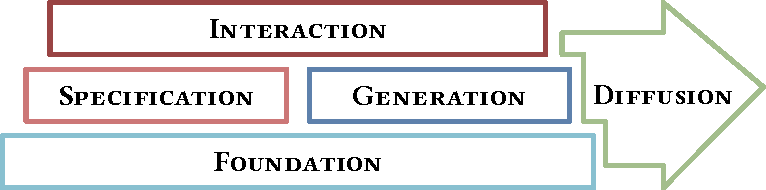
\includegraphics[width=.6\textwidth]{assets/overview.pdf}
  %\caption{Overview of the proposed research.}
  %\label{overview}
\end{wrapfigure}
%
We propose an interdisciplinary program of work on
{property-based testing}, bringing to
bear the combined power of PL and HCI to accelerate PBT's transition
into practice.
%
Planned research,
technology transfer, and education activities can be grouped into five main
themes: \iflater\bcp{Make sure this is an
  accurate summary -- e.g., the connection with fuzzing}\fi
%
\begin{enumerate}[noitemsep]
% \begin{itemize}[noitemsep]
% \begin{enumerate*}
\item We will establish a firm \thread{foundation} for HCI-informed research on PBT,
building on our past need-finding study and to confirm and generalize
its findings (\sectionref{sec:foundation}).
%
\item We will explore and apply a novel ``reflective'' approach to
\thread{generation}, enabling better generator tuning and counterexample
shrinking and linking PBT with fuzzing.  We will automate construction
of reflective generators, and we will construct a platform for
benchmarking these and other advances in tools for generation (\sectionref{sec:gen}).

% \item We will help developers efficiently define and tune random input
% \thread{generators} with novel techniques for generating values
% satisfying given preconditions, for test input mutation, and for
% example-based generator tuning---all building on a novel
% ``reflective'' approach to generation (\sectionref{sec:gen}).
%
\item We will empower developers to \thread{specify} properties with new
languages for expressing properties, tools that simplify authoring
properties, and assistants that help explain properties to others
(\sectionref{sec:spec}).
% tools for checking temporal properties over internal program states
% and for model-based testing of modularized code\proposecut{ and for authoring
% properties}, plus a comprehensive review of PBT practice to help
% students and developers identify situations where PBT is likely to be
% most useful\bcplater{the latter belongs under diffusion now, I
%   believe}
%
\item We will design, prototype, and evaluate novel tools for
\thread{interacting} with properties
and generators, leveraging our advances in specification and generation to
enable new ways of visualizing and understanding random distributions
over test inputs and pinpointing the cause of test failures.
(\sectionref{sec:val}).
%
\item We will support the \thread{diffusion} of PBT tools and
methodologies from academia into industry by supporting and
improving open-source PBT frameworks\iflater\bcp{multiple ones?  or
  should we focus better?}\fi{} and building a
comprehensive IDE for PBT, dubbed \tyche.
We will also drive diffusion via education, developing materials for teaching
software developers about high-value applications of PBT and
for introducing PBT into undergraduate and masters-level computer science courses
(\sectionref{sec:diffusion}).
% \amh{Our diffusion efforts will also amplify
% future research efforts through the creation and dissemination of reference
% implementations for others to build on, and an extensible development
% environment that future HCI researchers can extend with new PBT affordances.}
% \end{enumerate*}
% \end{itemize}
\end{enumerate}
%
Our goals for Broadening Participation in Computing are focused in two
areas: (1) expanding an
existing NSF-REU program that brings undergraduates from
underrepresented groups to Penn for summer research experiences in
programming languages, and (2) increasing diversity in the TA roster
for Penn's introductory computer science course, which PI Pierce
co-teaches.

\medskip

The rest of the Project Description describes this research and
technology transfer agenda in detail.  Sections
\sectionref{sec:orientation} and \sectionref{sec:motivation} supply
background on PBT and present preliminary findings from the
study at Jane Street.
%
Sections \sectionref{sec:foundation} through
\sectionref{sec:diffusion} outline plans for each of the
themes listed above.
Section \sectionref{sec:broader-impacts}
discusses Broader Impacts, and
Section \sectionref{sec:prior} summarizes our prior
NSF-supported work.

\SIMPLESECTION{Orientation: Property-Based Testing}{sec:orientation}
Developers in modern software ecosystems are often faced with code
that they do not fully understand. Applications are not cut from whole cloth;
they are built from large sets of components that are themselves often
assembled from multiple sources.
AI assistants like Copilot and ChatGPT make it even
easier to {\em get} code to carry out a given task but even harder to
{\em trust} that it is doing the right thing.

Property-based testing~\cite{hughes_quickcheck_2007} proposes an
effective approach to this problem---a straightforward way to evaluate
hard-to-understand programs is by validating them, semi-automatically,
against executable specifications. As a very basic example, a
developer might write the following function for checking that
the \lstinline{insert} function on binary search trees itself yields a new
binary tree:
\begin{lstlisting}
prop_insert_correct (x:int) (t:tree)  =
  if is_bst t then is_bst (insert x t)) else True
\end{lstlisting}
That is, if the tree passed to this function
is a BST, then it must remain
one after the insertion of \texttt{x} (where
\lstinline{is_bst} checks that its argument is a BST---i.e., whether it
is arranged so that each node's label is greater
than any label in its left subtree and less than any in its right
subtree).
%
In general, an executable property is a function that
accepts one or more generated
test inputs
and evaluates to \lstinline{True} if the test passes and
\lstinline{False} otherwise.
% This one, ``\verb|prop_insert_correct|'',
% checks that an insert operation on a binary search tree preserves the
% binary ordering of the tree.
Given such a property, a PBT tool generates a
large number of inputs and
checks that the property yields \lstinline{True} for each one; any input
that causes the property to fail is reported to the user as a
{counterexample}.
%
\amh{Not sure what the point of the next sentence is.} \proposecut{
Designing properties is an example of
the {\em oracle problem}~\cite{barr_oracle_2015}, which arises in any kind of
automated testing where the user needs to define what it means for a program to
be correct.}

The dominant approach to generating inputs (and the approach we focus on in this
project) is {\em random}
generation~\cite{hamlet1994random}. In contrast to enumerative
generation~\cite{DBLP:conf/haskell/RuncimanNL08, leancheck}, which iteratively
generates all possible inputs, random generation randomly samples inputs from a
potentially infinite distribution. The
surprising effectiveness of random generation can be attributed to the
``combinatorial nature'' of large test cases: bugs are
can sometimes exposed by any test input with a specific combination
of features, independent of the other features of the input. For example, a bug might be triggered by a particular
sequence of API calls in a particular order, even when
interleaved with other API calls. Random testing can sometimes
discover bug-triggering combintations of features more quickly than
exhaustive approaches, particularly those that begin with small inputs. Techniques like swarm
testing~\cite{groce2012swarm} can further amplify this effect.

\smallskip

To apply PBT to a software system or an individual component, the
developer first defines one or more properties that they expect the
system should satisfy.  They supply {\em random input generators} for
the values that the properties take as input---these are sometimes
written by hand, but often they can be automatically generated, e.g.,
from the type of the input. Next, they invoke the PBT tool to check
their properties against many generated inputs. And finally, if a
counterexample is discovered, they inspect it to determine the source
of the bug.  Each of these steps can be significantly improved for
users, as we describe below.

Why go to the trouble of using PBT, rather than the more straightforward
example-based testing that is standard across the software industry?
One reason is that it can exercise a system much more
comprehensively than a small number of hand-written examples.
% \proposecut{As mentioned
% previously, PBT has an impressive track-record uncovering bugs that other
% approaches had failed to
% find~\cite{arts2006testing,hughes2014mysteries,
% Bornholt2021,arts2015testing,hughes2016experiences}.}
But
PBT is more than just thorough---it is also more general than example-based
testing. For example, Wrenn et al.~\cite{wrenn2021using} observed that
{\em relational} correctness conditions (e.g., the fact that a program
topologically sorts a graph, which might
produce any of a number of correct results) cannot be represented
faithfully with example-based tests; a property-based specification is
a better choice in such cases.
%
PBT is also
a natural choice if
the developer already has some formal or semi-formal
specification in mind---for example if they are implementing behavior from an RFC or
other design document.
Finally, the
properties used for PBT can also serve as documentation of what a
program is supposed to do.

PBT is often compared to {\em fuzz testing}~\cite{afl-readme},
which randomly tests software to find
vulnerabilities. We discuss ideas for bringing PBT and
fuzzing closer together later in the proposal
(\sectionref{sec:reflectivefuzzing}), but current fuzzers have fundamentally
different goals from PBT.  In general, fuzzers need to run for a long time (hours or
days), they are commonly used to test whole systems ``from the
outside'' by provoking
crashes. Properties in PBT, on the other hand, can typically be
checked more quickly (on the order of seconds), they express richer
constraints on behavior than ``does not crash,'' and they can be used
to test both whole systems and smaller components.  Both techniques are useful, but
they are applied in different ways, at different points in the
development process, to achieve different goals.

With all these advantages, one might hope to find PBT on every
software developer's toolbelt.  But using PBT effectively
can be challenging, as we shall see next.

\iflater
\todo{Add a paragraph or two enumerating well-known / obvious
  challenges of PBT.  Then the next section begins ``We validated
  these challenges and added some color about additional ones that are
  not so much discussed in the PBT literature through a user study at
  Jane Street...''  }  \bcp{Or maybe it reads OK as-is?}
\fi

\SIMPLESECTION{Motivation: A Study of PBT in Practice}{sec:motivation}
\iflater\bcp{OK, I crunched this section down to a page.  I don't want to go
  too much shorter because it is doing a lot of work introducing the
  themes that we return to later...}\fi
%

Our research agenda is motivated by a deep formative study we conducted to
understand the state of the practice of PBT. This study will appear in 2024 on
the ICSE technical paper track~\cite{ref:goldstein2024property}.  In this
study, we partnered with Jane Street Capital to observe practice of PBT as it
manifested in a firm that sees substantive use across a wide variety of
software development settings.  The purpose was to identify the realities of
contemporary PBT practice and to critically examine what it might take to boost
adoption.

The study consisted of thirty semi-structured interviews with (1)
developers who use PBT and (2) maintainers of PBT tools. The study led to a
rich characterization of PBT benefits and pitfalls. While this characterization
is not complete---in that it represents experiences at just one firm---it does
represent the limits of what is possible among experienced programmers with
modern tools: Jane Street uses state-of-the art PBT tools, with integration of
the tools into much of the company's culture and tooling.  Here we report major opportunities the study revealed for transformative improvements to PBT tooling.  Our
upcoming need-finding work (\sectionref{sec:foundation}) will help complete the
picture of the potential impact of these improvements.

\iflater\amh{I removed the mention of the HATRA workshop paper because I could not think
of how to include it, though we may need to add it back in.}\fi

% We also carried out a
% smaller pilot study among Hypothesis users to prepare for the
% full-scale study at Jane Street; its results were presented at the
% 2022 HATRA workshop~\cite{goldstein_problems_2022}.

% Our choice of Jane Street as a partner was motivated by our desire to
% understand PBT in a non-academic setting where it is already broadly appreciated.
% At Jane Street, PBT is an
% established methodology, so there is a large
% population of people with well-informed opinions on its benefits and
% challenges. Additionally, Jane Street builds much of its
% software in OCaml, a functional language with
% a well-engineered PBT framework.
% %
% This unified
% ecosystem means that developers have access to mature PBT tools,
% experience using them in collaborative settings,
% and awareness of language-level abstractions necessary
% for expert usage of the tools.
% %
% All this makes Jane Street an ideal place for understanding the
% impact and challenges of PBT when users who have incentive to use
% it to full potential are provided with state-of-the-art tools.

\ifthemecolors\bcp{Make the colors here (if we're using them) match
  the ones in the timeline.  Also, we've got five main sections but
  only four colors here... is that confusing?  I think so.  Maybe
  better monochrome...} \fi
\newcommand{\proptheme}[1]{{\ifthemecolors\color{nord-orange}\fi \em #1}}
\newcommand{\gentheme}[1]{{\ifthemecolors\color{nord-green}\fi \em #1}}
\newcommand{\evaltheme}[1]{{\ifthemecolors\color{nord-purple}\fi \em #1}}
\newcommand{\edutheme}[1]{{\ifthemecolors\color{nord-frost4}\fi \em #1}}

% % \subsectionstar{Usability Challenges}\hg{Is this section header doing anything?}
% The final product from
% the ongoing study will be a fine-grained, qualitative description of how
% Jane Street developers use PBT, what they need from it, and how the
% research community can
% help improve it.  While the full analysis of the interview data remains
% to be completed, a number of themes are already clear; these
% % , together
% % with the findings of the preliminary study,
% form the backbone of the present proposal. We describe them below,
% italicizing themes and
% referring to evidence from participants in the Jane Street study
% (\participant{1--30})
% and the pilot study (Pilot-\participant{1--8}).

A first opportunity to advance the practice of is with new approaches for
\thread{generation} of random inputs. Developers spoke highly
of their tools' ability to \gentheme{derive
  generators} from data type specifications (e.g., by using ``\texttt{ppx\_quickcheck}''). At the same time,
they identified deficiencies both
small and large, the most significant being that derived generators
cannot enforce semantic preconditions like \lstinline{is_bst}.
%
When derived generators failed, participants fell back to creating
\gentheme{bespoke generators}, which are far more flexible but
proportionally more time-consuming to build.  Improving the
abstractions available for authoring such bespoke generators would
greatly improve the usability of PBT.
%
When generated inputs violate a property, developers often need to
inspect the input to understand it and how it triggered a violation.
Developers often
implemented their own \gentheme{shrinkers} for counterexamples to discover
simpler (and hence easier-to-understand) inputs that trigger the same bug.
%
But shrinkers need to be customized to particular kinds of data to be
most effective, and they can be time-consuming to build.

A second opportunity is to equip developers
with more powerful means to define properties, or \thread{specifications}.  PBT is often described as
a lightweight formal method, and one might therefore imagine that a
common challenge would be coming up with the specifications of desired
program behavior. Indeed, in our earlier pilot
study~\cite{goldstein_problems_2022}, developers with less experience
with PBT sometimes struggled to \proptheme{imagine properties} or to
understand what properties to test.  By contrast, Jane Street
developers on the whole reported little difficulty finding
properties. Rather, most developers applied PBT in
\proptheme{high-leverage scenarios} where properties were already
available or straightforward to invent.  This suggests that an
effective way to boost PBT in industry would be to provide educational
materials and documentation that highlight real-world applications
where it is a natural fit.
%
We also heard \proptheme{opportunities for better leverage} of
specifications, where PBT is not easy {\em yet} but could be with a
bit more research effort.  In particular, better automation and
tooling around {\em model-based testing} appears to be an excellent
way to improve PBT usability.

A third opportunity is to give developers more powerful
\thread{interaction} mechanisms to inquire about their tests'
effectiveness
and influence their behavior. Developers often relied on ad hoc,
piecemeal approaches to \evaltheme{evaluating the effectiveness} of their
tests. Many wished for better ways to evaluate their generators and
properties, including feedback on code coverage, mutation
testing~\cite{papadakis_mutation_2018}, and help understanding the
distribution of randomly generated inputs. Novel ways of visualizing
test effectiveness could in turn provide new ways of enabling the
manipulation of distributions of generated inputs.

Finally, our study conveyed that \thread{diffusion} of PBT tended
to take place with the advocacy of tool builders and users. We reflect
on the fact that for PBT to reach into new organizations and new teams
within organizations, it will likely investment in developing more mature cultures that
teach its power and usage. PBT is
not taught in traditional computer science curricula at the
undergraduate or masters level; making more developers aware of it
will required expanded \edutheme{classroom education}.
%
And finally, existing tools for PBT need continual support to meet
demands from growing (and increasingly sophisticated) user-bases; to
help PBT move into the mainstream, we should look for high-value ways
to improve \edutheme{open-source PBT frameworks} with the insights and
tools we develop.

% Several sets of themes emerged from this study.  One concerned the \thread{generation} of
% random inputs for PBT. Developers spoke
% highly of the \gentheme{Derived Generators} that can be automatically
% inferred from
% the OCaml type system (\participant{5} called OCaml's implementation of this
% ``[expletive] amazing'' and \participant{30} called them a ``game changer'').
% These generators are already quite good, but they could be better: participants
% identified deficiencies both small and large, the most significant being that
% derived generators
% cannot enforce semantic preconditions like \lstinline{is_bst}.

% When derived generators
% failed, participants fell back to \gentheme{Bespoke Generators}, which
% are far more flexible but proportionally more time-consuming to
% build. For example, \participant{20} successfully used a bespoke
% generator for XML documents to find significant bugs in their code,
% but reported spending ``at least a day'' writing it.
% Improving the abstractions available for authoring bespoke generators would
% greatly improve the usability of PBT.
% %
% When a generated input turns out to be a counterexample that triggers
% a property violation, the developer will need to inspect that
% counterexample to find
% and fix the root problem. Developers often implemented code for
% \gentheme{Shrinking} counterexamples to discover
% simpler inputs that trigger the same bug.  \participant{8}
% and \participant{21}, who each implemented their own PBT frameworks, both
% incorporated shrinkers as key components. But
% shrinkers need to be customized to particular kinds of data to be most
% effective, and they can be time-consuming to build; several
% developers
% (\participant{16}, \participant{20} \participant{21}, \participant{30})
% described constructing shrinkers as an opaque and difficult process.

% A different set of themes
% themes revolves around properties themselves, i.e.,
% \thread{specifications}.
% % and the kinds of programs in which they choose to test them.
% PBT is often described as a lightweight formal method, and one
% might therefore imagine that a common challenge would be coming up with the
% specifications of desired program behavior. Indeed, in our earlier pilot
% study~\cite{goldstein_problems_2022}, some respondents indicated just that:
% developers with less experience with PBT
% sometimes struggled to \proptheme{Imagine
% Properties} or to understand what properties to test (Pilot-\participant{1},
% Pilot-\participant{3--5}).
% By contrast, Jane Street developers on the whole reported
% little difficulty finding
% properties. Rather, most developers applied PBT in
% \proptheme{High-Leverage Scenarios} where properties were already
% available or straightforward to invent. In the words of
% \participant{9}, PBT is particularly easy to apply
% when
% one has ``a really good abstraction with a complicated implementation.''
% When asked to speculate, several participants (\participant{3}, \participant{15},
% \participant{20}, \participant{22}) guessed
% that 80--100\% of Jane Street
% developers write programs like this,
% % \bcplater{Did anyone really guess
% %   100\%??}\hg{Yep! Someone said ``everyone.''}
% where properties are easy to find and
% PBT is relatively easy to apply. This suggests that an effective way to
% boost PBT in industry would be to provide
% educational materials and documentation that highlight
% real-world applications where it is a natural
% fit.

% We also heard \proptheme{Opportunities for Better
% Leverage} of specifications, where PBT is not easy {\em yet} but
% could be with a bit more research effort. For example, developers in
% both studies (Pilot-\participant{4--6} and Jane Street \participant{7}) complained
% that PBT was difficult when code was poorly abstracted.  Further,
% more than three
% quarters of study participants had used a particular approach to PBT commonly
% called \proptheme{Model-Based Testing}.  \participant{3}, an author of PBT tools
% at Jane Street, considered better automation and tooling around model-based
% testing to be one of the most significant ways to improve PBT usability.


% A further set of themes concerned the
% \thread{interaction} between developers and their
% testing environments---especially their strategies
% for \evaltheme{Evaluating the
% Effectiveness} of their tests. Many
% wished for
% better ways to evaluate their generators and properties, including
% feedback on code coverage (\participant{9} and \participant{25}),
% mutation
% testing~\cite{papadakis_mutation_2018}, and help understanding the
% distribution of randomly generated
% inputs (\participant{10}, \participant{16}, \participant{16}). Worryingly,
% while many developers admitted they would benefit from better ways to
% evaluate their tests, many seemed to
% \evaltheme{Implicitly Trust the Infrastructure} that they did use. \participant{14} actually shipped broken code because
% they did not realize their generator had missed important cases.
% Additionally, one participant (\participant{14}) saw significant benefit from
% \evaltheme{Visualizations} they had built themselves to
% understand their testing effectiveness.

% Finally, our experience with these studies (and with the products of
% our own prior research!) suggests
% that significant engineering and pedagogical effort is needed to amplify
% PBT's \thread{diffusion} into the broader community.  Developers in both studies
% (Pilot-\participant{1}, Pilot-\participant{4}, JS \participant{3} and
% \participant{11}) reported a dearth of \edutheme{Documentation and Examples} for
% learning about PBT.  PBT is also not
% taught in traditional computer science curricula at the undergraduate
% or masters level; making more developers
% aware of it will required expanded
% \edutheme{Classroom Education}.
% %
% Finally, existing tools for PBT need continual
% support to meet demands from growing (and increasingly sophisticated)
% user-bases; if PBT is to become mainstream, we should look for high-value
% ways to improve
% \edutheme{Open-Source
% PBT Frameworks} with the insights and tools we develop, to help our
% work and ideas permeate the PBT world.



\SECTION{Foundation}{Understanding Needs and Opportunities%
\pagebudget{1}}{sec:foundation}

\bcplater{I tried to make the opening of this section give a better sense
  of why we think the preliminary study is a useful motivation for our
  research even if it's ``just about Jane Street'' and needs to be
  fleshed out to learn about other settings.  But maybe it repeats too
much from the top of section 2...?} \amh{I tried simplifying below. I think the justification may be less necessary after my recent revisions to Section 2}

Our program of research begins with broadening and deepening our view of PBT,
how it takes place, and the opportunities for transformative change. Our first
step in this process is described in the prior section, with our deep qualitative
study of use of mature PBT tools among experienced engineers. Our next steps
will be to develop an account of PBT that is both \emph{broad}---i.e., representing
more developers, in more development contexts---and \emph{deep}---i.e., descriptive
of the tasks that programmers in a way that can support design decisions
in the development of new algorithms and interfaces.

% The findings of this industry study paint a clear
% picture of both the benefits and the challenges of PBT for
% Jane Street and other software development organizations with similar
% characteristics---teams consisting mostly
% of relatively skilled developers who are comfortable with
% advanced programming languages and tools and who care a lot about
% software correctness.  There are many such teams in the software
% world, and making PBT more
% usable for them would already be a significant step in the
% right direction.  But to
% understand potential impact of PBT
% across the {\em  whole} software
% industry---and the factors that may limit its adoption---we need to
% cast a wider net.

In this section, we describe a further plan of user research that will
establish a {\em foundation} for the latter stages of this project, as well as
the broader PBT research community. This research will follow rigorous HCI methods.
We will ensure fairness, ethics, accountability, and transparency (FEAT)
by developing our study plans in consultation with Penn's Institutional Review Board (IRB).

% Building a
% rigorous foundation, with methods motivated by the HCI literature, is substantial work,
% but it will significantly increase the chance that future projects achieve their goals.
% We plan two
% written surveys, one to assess the generality of these needs and obstacles
% and one to identify potential for adoption of PBT tools
% (\sectionref{sec:survey}) and two user studies, a design probe using a minimal
% PBT framework
% and an observation study
% to guide the design of
% interactive tools
% (\sectionref{sec:observations}). Finally, we plan to distill these
% study findings into a cognitive
% theory of property-based testing, a conceptual foundation for the
% design activities elsewhere in the project (\sectionref{sec:cogtheory}).
% The projects in this section will culminate in an article for the Communications
% of the Association for Computing Machinery (CACM).
%
% To ensure fairness, ethics, accountability, and transparency (FEAT),
% each of our user studies will be vetted through Penn's Institutional
% Review Board (IRB) review process.

\SUBSECTION{Developing a broad understanding of needs and opportunities}%
   {sec:survey}{1}{1}{HCI Theory}{PhD 1}{REPL 1}{Head}
%
Our prior interview study revealed a rich
set of opportunities to improve property-based testing. As noted above, the interview
study sampled developers at one firm with a mature testing culture and PBT toolset.
While this is enough to indicate the upside of myriad kinds of improvements
to PBT, there is considerable value to be had in completing the story with
the broader population of developers. 
We will therefore conduct two surveys with the goals of (1) validating and
extending our inventory of opportunities found in our first study and (2)
understanding the potential upside of better tools for the
software industry.

% Our industry study has already revealed
% a number of
% opportunities to improve property-based testing. To identify
% others and to better understand which are most
% critical, we will conduct two
% surveys with broader samples of developers. These surveys aim to
% (1) determine which obstacles observed in the original
% study
% represent widely experienced pain points and
% (2) understand the potential benefits of better tools for the
% software industry.

The first and larger survey
aims to understand the degree to which
the findings of the Jane Street study generalize to other settings.
We will
ask developers which of the issues we identified there are
ones they have also encountered, which are most severe
in their experience, and what
other issues they have encountered.
To provide
clear usage scenarios, respondents will
be asked to write brief anecdotes elaborating on the
most severe issues they remember.  Other questions will assess how
heavily respondents depend on specific features of their PBT tools
that may be enabled by their
ambient programming environment and language, e.g., whether the
language supports Haskell-like typeclasses or OCaml-style
metaprogramming, both of which are used to good effect by
PBT tools in those languages.
\iflater\bcp{Is this sentence needed?}\fi{} In line with typical practice in
human factors research surveys in software
engineering~\cite{ref:robillard2009makes,ref:uddin2015api,ref:murphyhill2019predicts},
we will recruit at least 150 respondents per survey.
Respondents will
be recruited broadly, from groups including
(1)
users of the major PBT frameworks in Python, Java, Haskell, Rust, and
Scala, capitalizing on our personal connections to maintainers of
these projects (and in particular Zac Hatfield-Dodds of Python's Hypothesis; see attached letter of support); and
(2) our own and our students' professional networks, including
Twitter and Mastodon, mailing lists, and discussion boards for developer
conferences---e.g., ``Yow!'', where PI Pierce spoke last
year~\cite{Pierce:Yow22}.

% \TASK{Impact survey}{2}{2}{Who?}
A second survey later in the project will investigate
how broadly PBT may {\em eventually} be able to reach.  We will
survey developers who do {\em not} use PBT
currently but who might find it particularly useful.
We will again recruit a broad sample of participants from varied settings.

\publicationtarget{International Conference on Software Engineering (ICSE)}

% \SUBSECTION{Dimensions of PBT infrastructure design}%
%   {sec:frameworks}{3}{4}{HCI Theory}{PhD
% 1}{PhD 4}{Head}
%

% \bcp{I am not really convinced by this yet.  What are these
%   ``dimensions'' where we are going to choose between alternative A
%   and alternative B?  Integrated vs. external shrinking, sure, but
%   after that, what??  If we can list four or five key dimensions, we
%   should.  If not, maybe drop this task?  (I'm also worried about how
%   easy it's going to be to implement a new PBT tool that embodies all
%   possible combinations of these choices, much less in a ``minimal''
%   way...)}\hg{I listed three, internal vs external shrinking, maximal vs minimal
%   generator automation, and bespoke property language vs. just write a Boolean
%   function. I imagine we'd find more if we actually did the study... My goal
%   with this project would be to have an empirical basis on which to say ``hey
%   QuickCheck, let's just implement internal shrinking'' and ``hey Hedgehog, you
%   may want to give users better generator automation.'' It's consistently
%   frustrating when a library in one language is strictly better in one way, and
%   one in another language is better in another, and it has nothing to do with
%   the language}

\SUBSECTION{Observational studies}{sec:observations}{2}{2}{HCI
    Theory}{PhD 1}{REPL 2}{Head}
\bcplater{Wonder whether there is still room for cutting / compressing
  here...  If the project only has two students, we may not want to
  propose {\em too} many studies...}%
%
Interviews and surveys are good for exploring usability challenges
at a high level, but we also need detailed insight into the interactions
between users and their PBT tools.  We will
conduct targeted observational studies, in particular to inform our
user interface designs (\sectionref{sec:val}).

% Understanding user interactions
% is a core activity of HCI research and helps to inform robust
% interface design.
Observation studies require significant effort to plan and
carry out, but they
are indispensable for answering questions about tool design may that
receive only
speculative answers in interviews and surveys, such as
(1) How much time
are participants willing to devote to
creating a property or tuning a generator when in the
middle of a programming task?
(2) How much space is available on a developer's
screen (amidst other tools like code editors and terminals) for
new live
visualizations? and
(3) What are developers' current strategies for solving the
problems they describe, e.g., what representations
seem helpful
for a programmer trying to understand the distribution of data from a
generator?

We will conduct two studies. The first will be a
{\em contextual inquiry}~\cite[Chapter
3]{ref:holtzblatt1997contextual}, watching
developers perform PBT in realistic contexts, with their own tools and tasks.
The result will be a detailed understanding of the task
structures involved with specific PBT tasks (e.g., writing a generator,
assessing test results) and what steps are
particularly time-consuming.  Recordings and notes from
these sessions will serve as metrics against which designs
can be evaluated before implementation.

The second study will be a controlled comparison of design alternatives.
Language design, like what we plan relating to generators
(\sectionref{sec:reflectiveusable}, \sectionref{sec:genauto}), is famously
difficult to inform empirically because there are many design choices
that interact in complex ways. We plan to identify the most
significant patterns of
variation between modern PBT tools (e.g., defining properties as simple
functions vs. via DSLs, or using types to steer
generation vs.{} fully manual generators), and perform a comparative
study to gain clarity on how various
choices would impact our design. Following best practices in experiment design
for programming tools~\cite{ref:ko2015practical}, we will keep the experimental tasks simple, train
participants to control for variance in prior skill, and triangulate findings
from a mixture of
quantitative metrics (e.g., success, task duration, error rate, subjective
reports of difficulty) and qualitative analysis (e.g., thematic
analysis~\cite{ref:blandford2016qualitative} to reveal the kinds and frequency
of problematic incidents).
\proposecut{Most of these findings will be in service of research projects described elsewhere
in this proposal, but they may also be disseminated as
publications if they turn out to be of broader interest.}

\publicationtarget{PLATEAU Workshop}

% \SUBSECTION{A cognitive theory of PBT}{sec:cogtheory}{2}{3}{HCI
%   Theory}{PhD 1}{Everyone}{Head}
% %
% % A cornerstone of our efforts to bring PBT to people in industry
% % will be a new cognitive theory of PBT itself.
% Theories of
% programming have
% long served a critical role in human-centered software engineering
% research, providing rich and memorable descriptions of programming
% processes and clarifying opportunities to improve tooling and training.
% For instance, Lawrance et al.~\cite{ref:lawrance2010programmers} advocate for the use of {\em information foraging
%   theory}~\cite{ref:pirolli2003exploring} to
% describe how programmers navigate complex code bases to search for behaviors
% within that code. This
% theory has motivated a variety of tools that demonstrably improve the
% programming experience (e.g.,~\cite{ref:henley2014patchworks}).  Other theories
% that have inspired advances in programming tools include
% Blackwell's Attention-Investment model~\cite{ref:blackwell2002first} Ko and
% Myers' debugging framework~\cite{ref:ko2005framework}, and Ko's characterization
% of end-user programming barriers~\cite{ref:ko2004six}.

% Recognizing the power of theory, one of the first steps in our
% research will be to develop a cognitive theory of PBT. The starting point
% will be the conceptual framework we are developing through the Jane Street study. This
% will be validated and refined with evidence from early observation studies we
% described in~\sectionref{sec:observations}, leading to a
% provisional theory in the first two years.
% This theory will help us
% refine our ideas for
% tools and provide a foundation for contextualizing the questionnaires and
% observations described in the following sections. Conversely, evaluations of
% the tools we build will provide additional evidence to further
% refine the theory.

% A successful outcome of this effort will be a
% theory that is simple, evocative, and validated. The theory will
% define the constructs involved in PBT,
% including the tasks involved in PBT (e.g., generation, property specification,
% and reviewing test output) and a developer's goals (e.g., developer time, test
% speed, and level of assurance). It will explain tensions between goals (e.g.,
% more assurance often means more developer time). Furthermore, it will identify
% how developers make choices to achieve their goals. For instance, our Jane
% Street interviews showed us that some developers' testing activity
% might better be described as
% satisficing~\cite{ref:brown2004consideration} rather than maximizing
% assurance of a system: these developers limited the time they spent
% writing and running tests, although more testing effort might well have
% revealed further bugs or achieved better coverage. A theory that brings
% these elements together would suggest that for such developers to
% achieve higher assurance, they would evidence that better assurance is
% possible with only modest effort.

% \publicationtarget{Foundations of Software Engineering (FSE)}

% \smallskip The projects in this section will develop an evidence-based model for
% PBT that will be useful far beyond our research. Therefore we also plan to
% publish an article in the Communications of the Association for Computing
% Machinery (CACM) to communicate about PBT to a broader computer science audience.

\SECTION{Generation}{Better Tools for Random Inputs\pagebudget{3}}{sec:gen}
Many of the usability challenges revealed by our industry study concern
around test input
\gentheme{generation}.
Indeed, generators were regularly cited as one of the most challenging
aspects of PBT.

We propose a number of extensions and applications of {\em reflective
generators}, a new abstraction for random generation that
``unbundles'' generator
functionality, exposing levers for
automation that enable a number of new approaches to generator
tooling. We explore how reflective generators can
help to connect PBT and fuzzing (\sectionref{sec:reflectivefuzzing}),
and we design
a user study for evaluating and improving the usability of reflective
generators (\sectionref{sec:reflectivepeople}). Finally, we discuss
plans to boost generator automation (\sectionref{sec:genauto}) and metrics
by which to evaluate improvements in generation (\sectionref{sec:benchmarks}).
Success for these enabling technologies will be measured both by the success of
the tools built on them (\sectionref{sec:val} and \sectionref{sec:diffusion})
and by top-tier publications, including performance evaluations and/or
user studies as appropriate.
PI Pierce is a longtime collaborator of John Hughes, one of the
QuickCheck creators, who plans to collaborate on the projects
in this section; a letter of collaboration from Prof.{} Hughes appears
in the supplemental documents.

\subsectionstar{Context: Why Random Generation is Hard}{}{}
As discussed in \sectionref{sec:orientation}, PBT relies heavily on {random data
generators}.  Checking a property for many randomly generated inputs
gives confidence that it holds---{\em provided} the inputs actually
exercise a wide variety of program behaviors.
Unfortunately,
many properties of interest have {\em preconditions}
({a.k.a.} {validity conditions} or {input constraints})---for example,
the \verb|prop_insert_correct| function above succeeds trivially unless
\verb|is_bst| holds of the input tree.  Such precoditions come up in
practice, and they are problematic because they can be
difficult to satisfy randomly, so most of the testing budget
can be wasted generating and discarding precondition-failing inputs.
%
\proposecut{(Of course, some fraction of the testing budget {\em should} be spent on
ill-formed or nonsensical inputs, but not too much, since these will not
exercise much of the system's functionality; most tests should be
well formed---though perhaps unusual---instances of the sorts of inputs the
system is designed to process.)}
%
Worse, even generators that are guaranteed to produce valid
inputs can underperform in other ways---for example, by
generating many very similar inputs while ignoring large parts of
the input space.

Approaches to these challenges
fall on a spectrum from automatic to manual. The automatic approaches use
various proxies for validity and ``interestingness'' of
inputs: some, like {\em
fuzzers}~\cite{afl-readme}, try to maximize readily available metrics like code
coverage, while others ask users to provide their own metrics~\cite{loscher2017targetedpbt} and
some use machine learning to infer proxies for
validity~\cite{godefroid2017learn, DBLP:conf/icse/ReddyLPS20}. These approaches
are easy to apply and produce diverse sets of inputs, but they are rarely
sufficient for testing properties with complex
preconditions because too few of the inputs they generate are
valid. Slightly more
manual approaches are based on declarative representations of validity
conditions: for preconditions that are primarily structural, {\em grammar-based
fuzzing} provides a compelling solution~\cite{godefroid2008grammar,
holler2012fuzzing, veggalam2016ifuzzer, wang2019superion,
srivastava2021gramatron}, and for more complex, semantic preconditions,
SMT-solvers~\cite{dewey2017automated, beginners-luck,
steinhofel_input_2022} can be used to automatically seek out valid
inputs. These tools are
much better at satisfying easy to moderately complex properties but
much worse at very ``sparse'' properties. The semi-automatic
category also includes tools for {\em example-based tuning}, a process that
improves realism of inputs by mimicking user-provided
examples~\cite{soremekun2020inputs}; these tools can generate
realistic inputs, but they are again limited to structural preconditions.

The most flexible, most manual solutions use hand-built
generators, often written in a special-purpose domain-specific language (DSL).
Such DSLs are often implemented using {\em
monads\/}~\cite{moggi1991notions}, an elegant design pattern for
expressing effectful (here, random and stateful) computations\proposecut{
in a pure, stateless underlying
language}. \proposecut{While monadic DSLs are not
needed to express generators in
impure languages, some frameworks (e.g., in OCaml) still choose to use monadic
abstractions for their generator DSLs.

\smallskip
}Monadic generators can implement random data producers of arbitrary complexity
(e.g., generators for for random Haskell
programs~\cite{palka_testing_2011}); in this sense, they are strictly more expressive than
representations like grammar-based generators.  Yet monadic generators are
syntactically constrained in a way that isolates the probabilistic code and
prevents usage errors (like passing the wrong random seed around).

We can further improve monadic generators by re-framing them as {\em
  parsers of random choices}. The usual intuition is that a generator
operates by making a series of random choices, but we can think of
it as being {\em given} a random sequence of choices and following
those choices to produce a value. This shift of perspective has been
used as the basis for past implementations of PBT
tools~\cite{maciver2019hypothesis, dolan2017testing}; we were the
first to make it
formal using {\em free generators}
in our paper, {\em Parsing Randomness}~\cite{goldstein2022parsing}.


\subsectionstar{Context: Reflective Generators}{}{} Building on the
idea of free generators, we are now exploring a powerful
generalization called {\em reflective
  generators}.  The basic concept came out of a
past NSF project (see \sectionref{sec:prior}). Our first paper on
reflective generators won a distinguished paper award at ICFP 2023.

The special thing about reflective generators is that they can be run
{\em backward}.
If running a generator in the usual way can be seen as parsing a
sequence of choices into a
value, then running it backward takes that value and produces a
sequence of choices that
would generate it\proposecut{---i.e., reflective generators can
``reflect'' on a given test and analyze the choices that they
could have made to generate it}.
The mathematical machinery
involved is somewhat complex,%
\footnote{\normalsize Reflective generators are both monads and {\em
    partial profunctors},
implementing bidirectional programming in the style of Xia et
al.~\cite{xia2019composing}. This approach to bidirectional programming is
related to lenses~\cite{foster2009bidirectional}, but it hides much of the
complexity of bidirectional program composition in the bind operation of the
monad, allowing both directions of
the computation can be written at once, in a type-safe way.}
but, as with free generators, the syntax that users see remains close to
that of normal monadic generators.

Running a reflective generator backward is not simply a matter of
remembering the choices it made going forwards and replaying them in
reverse order (as some PBT frameworks already do~\cite{maciver2019hypothesis,
  hatfield-dodds_hypofuzz_nodate}). For one thing, a reflective
generator can reflect on inputs it did not actually
produce---all that's required is that it {\em could} have produced
them.  For another, the choices can be structured in different ways (as bit
strings, higher-level choice sequences, choice trees, etc.) if increased
structure reveals information that an analysis algorithm (like the ones
discussed below) can use. \iflater\bcp{Don't understand that sentence.}\fi{}

Reflective generators have myriad uses. First,
%
it is often helpful to start by testing with
``realistic'' inputs that trigger common-case behavior in the program;
one way to ensure this is to tune the generator so
it produces values that are similar to some user-supplied values deemed
realistic. Existing tools make good use of this example-based approach to
tuning~\cite{soremekun2020inputs}, but they do not work with generators as
powerful as monadic generators. We have implemented a
similar algorithm using
reflective generators; with it, we can (1) reflect on realistic values to
obtain sets of choices, and (2) run the generator with {\em new choice weights}
informed by the choices that we saw. Our evaluation shows that reflective
generators approximate the performance of the algorithm
from~\cite{soremekun2020inputs} but work with a larger class of generators.
%
Second,
reflective generators can also be used as a tool for analyzing and
manipulating the structure of generated inputs. Inspired by the test-case
reduction algorithms in Hypothesis~\cite{maciver_test-case_2020}, we implemented
validity-preserving {\em shrinking} of values to find smaller counterexamples
and speed up debugging with no additional effort from the user.%
%
\footnote{%
\normalsize
Hypothesis shrinks test inputs by shrinking the random choices
that produce those
inputs. This means shrinking can be implemented
generically, and it can leverage the generator code to ensure that shrunk
inputs are valid with respect to property preconditions.  But shrinking
random choices requires that these choices are actually available, which
is not always the case. Reflective generators
can
recover the random choices and thus enable shrinking
on any
valid input, not just those that we know the choices for.  We can, for
example, shrink inputs provided by the developer or
gleaned from bug reports.  \iflater\bcp{Wonder if that is getting too much
  into the weeds...  Maybe cut this footnote?}
\hg{Don't we need to say this somewhere?} \bcp{I reckon so.  Maybe we
  can find enough things to cut elsewhere...}\fi}
%
And third, reflective generators can be freely
``reinterpreted'': the same code that specifies random choices can
also be used to {\em enumerate choices} or make {\em dynamically guided choices}.
\proposecut{As new strategies for guided random generation and
enumeration become available, they can be used to improve reflective
generators.}

\SUBSECTION{Algorithmic advances for reflective generators}{sec:reflectivefuzzing}{1}{1}{PBT
  Theory}{PhD 2}{Engineer}{Pierce}
%
The response to reflective generators has been encouraging (the paper
introducing them was named a Distinguished Paper at ICFP 2023), but
this paper only scratches the surface when it comes to building and
evaluating potential use-cases.

First, we believe more powerful approaches to example-based tuning are
within reach.  The
``Inputs from Hell''\iflater\bcp{first mention!}\fi algorithm used in
our initial evaluation assumes
that subsequent choices are
independent of earlier ones, tracking the weights of individual
choices independent of the
context in which those choices are made. If we really want to mimic an existing
distribution of values, we should take that contextual information into
account. We propose modelling choices and their contexts via a neural network,
rather than a simple distribution map, compressing the data into a compact
representation that is easy to query.
This should make the example-based tuning
procedure far more accurate, allowing it to much more faithfully replicate
important features of complex input sets.

Beyond example-based tuning, reflective generators are a compelling opportunity
for integrations with
{\em fuzzers}~\cn \hg{See Shriram's comments on the ICSE paper for stuff on this
citation}. Fuzzers manipulate their distributions over time, not based on
user-provided examples, but instead based on live feedback about coverage of the
code under test.
Some existing projects have already worked to
combine PBT and fuzzing.
For example, the FuzzChick framework in Coq~\cite{DBLP:journals/pacmpl/Lampropoulos0P19}
uses code coverage as guidance for PBT, and HypoFuzz uses a
similar approach in Python~\cite{hatfield-dodds_hypofuzz_nodate}. These projects
are demonstrably powerful, but neither benefits from the years of expertise
poured into industrial-strength fuzzers; the Crowbar testing tool in
OCaml, on the other hand,
does~\cite{dolan2017testing}. Crowbar re-purposes
AFL~\cite{afl-readme}, one of the best-established
fuzzers: instead of letting AFL directly generate program inputs, it
uses AFL
to generate a sequence of choices that a generator then parses to get a program input.
This scheme
does require the user to write a generator, which is more effort
than standard fuzzing, but the result is a system that is much more likely
to achieve thorough testing\bcp{@Harry: do we have evidence for this}.

We believe this idea can be pushed even further by building
a variant of Crowbar on top of reflective generators.
The idea of crowbar is to start with a classic fuzzing setup, which tries to make the
system under test
crash by passing it a variety of semi-random inputs. But instead of
the fuzzer
``working against'' the parser, in the sense that the parser's job is to reject
invalid inputs and the fuzzer's job is to get past it, Crowbar's generators are
monadic and can generate
inputs that always pass the parser. Our generators will be monadic for the same
reason, but also {\em reflective}.

Why a reflective generator?
To start,
because its backward interpretation can be used to seed the fuzzer.
Modern fuzzers often
ask the user for a number of {\em seeds}---examples that the fuzzer
can start from,
to ensure that it does not spend ages exploring
inputs that have no hope of getting beyond the parser in the system
under test and exercising other parts of the system. Normally these
seeds are easy
for the user to write down---they are just program inputs---but
it is infeasible to ask the user to write down the sequences of choices that
result in their seed values.
This is one excellent use for a
backward interpretation. The user can write down their seeds---either as values
in the program, or as text that can be parsed by the program's parser---and
ask the reflective generator to get the choices that lead to those seeds.

\proposecut{
Regarding shrinking, the shrinking algorithm used in Hypothesis is powerful,
but not obviously optimal. Hypothesis shrinkers reduce the input
randomness to the
{\em shortlex smallest} choice sequence---that is, they favor
sequences that make the
generator make as few choices as possible, and where each choice is
``minimal.''  This is a useful heuristic, but it is not directly
related to the user's understanding of the size of the shrunk
inputs. Ideally, we'd like some
reflective shrinkers to {\em always} produce inputs that are smaller by some
natural metric on their type, not on the random choices that produced them; we
will state and prove the properties of a generator that imply this
property. \bcp{That ends a bit abruptly...}\hg{I didn't have much to say here.
  We can chop this paragraph if it doesn't feel useful}
\bcp{Chopped---we need the space.}
}

\hg{We're also missing publication targets, which might make it less abrupt}

\SUBSECTION{Reflective generators for the people}{sec:reflectivepeople}{2}{2}{PBT
  Theory}{PhD 2}{Engineer}{Pierce}
%
We would like reflective generators to be incorporated in
real PBT frameworks.
%
However, it is unclear
how reflective generators can be
represented in languages with weaker type systems than Haskell's. In
Haskell, the type checker can automatically catch many
common user errors, but this checking relies heavily on type-classes that
quantify over ``higher-kinded types'' (e.g., the monad type class). If
we hope to implement
reflective generators in frameworks like Python's Hypothesis library, we need to
design a programming discipline that makes the process equally safe and
intuitive. We plan to build on prior work exploring how to implement data structures
like monads in imperative
languages~\cite{brachthauser_representing_2021, delaat_pymonad_nodate} to design
a form for reflective generators that is appropriate in languages like
Python, Java, and Rust.

Another barrier to adoption is the extra work involved in turning a standard
generator into a reflective one\proposecut{, since reflective generators are unavoidably a
bit more complex than standard QuickCheck generators}. \proposecut{The current design of the
reflective generator language is a best guess at what users will find most
usable (based on our own experience), but we can do better than guessing!}
We will evaluate and redesign the surface syntax of reflective generators with
the help of real users, in a style informed by prior work in the HCI
literature~\cite{ref:ko2015practical}.  We will recruit a small group of users, teach
them to use reflective generators via a short ``README,'' and ask
them to implement a number of PBT generators inspired by the research
literature and real-world examples. We will both observe and interview
the users to identify points of friction and ensure a clear understanding of their
impressions. With this information in hand, we will identify potential changes
to the API and test those changes with a new group of users.  The
ultimate measure of success (again, evaluated through user interviews)
is whether our language for reflective generators is usable by non-expert PBT
practitioners.

\proposecut{%
Even with an ergonomic and learnable language for reflective generators, the
less code the user has to write the better. Both of our past user studies
revealed
that thinking about generators slows users down and makes PBT more challenging.
% But we should not compromise: any automation should help users obtain {\em high
% quality}, {\em reflective} generators for use throughout the testing process.
}

We will adapt existing tools for type-based generator
automation~\cite{mista2019deriving} to work with reflective generators.
\proposecut{In general, type-based
generators are only useful for testing properties with easily satisfiable
preconditions, but this is a good starting point for many developers.}
We will also consider techniques for {\em interactively}
constructing reflective generators that maintain complex preconditions.
% Some users may already have a standard QuickCheck-style generator that
% they would like to use
% in a situation that requires a reflective generator.
We will assist
users in generalizing existing generators to reflective ones, with tools that automatically synthesize backward annotations
required to make the generator bidirectional. We will experiment with both
conflict-driven program synthesis~\cite{feng_program_2018} and solver-aided
synthesis~\cite{torlak_growing_2013} to see which more successfully generates
the required annotations for realistic generators.

We plan to collaborate in this effort with professor Hila
Peleg at the Technion, who has experience with both PBT and program synthesis. A
letter of collaboration from Prof.{} Peleg appears in the supplemental documents.

% Going one step further, we will explore techniques that can synthesize an
% entire reflective generator from whole cloth. There are a variety of
% attempts to do this for standard generators: Lampropoulos et al. provides
% two solutions, one based on on inductive relation specifications of
% preconditions~\cite{Lampropoulos&18} and the other based on an
% extended language for properties~\cite{beginners-luck}, while Steinh\"ofel et al.
% infer a generator from constraints using
% Z3~\cite{steinhofel_input_2022,de_moura_z3_2008}.
% But none of these
% tools fully solves the problem of automated constrained generation in
% general, and none of them include the tools necessary to produce reflective
% generators.

% Pushing forward with generator automation could also extend the reach of PBT
% into new domains. Constrained generation is a major difficulty of the
% QuickChick ecosystem~\cite{paraskevopoulou_foundational_2015}, and automated
% generator solutions could be used to test program
% logics~\cite{jung_iris_2018,leino_dafny_2010} to improve usability of PBT in
% contexts like proof assistants. More generally, generator automation could make
% PBT viable in any situation where properties already exist but preconditions
% are hard to satisfy.

\SUBSECTION{Generator benchmark suite}{sec:benchmarks}{1}{1}{Tech
  Transfer}{REPL}{PhD 1}{Pierce}
%
% \bcp{Core ETNA is done.  Talk about future expansion -- e.g., into
%   Python, OCaml, so that we can robustly evaluate tools that have not
%   been considered in this way so far...  Talk about the ``acceptable
%   latency of benchmarks'' by analogy with jane street findings...}%
%
\bcp{Benjamin mentioned that there may be additional
    interesting things to do in the benchmarking space  [Benjamin and Harry]}%
Most papers in the existing PBT literature use small case studies,
showing that certain bugs in certain systems
are caught more quickly with their tool than existing ones. For
theoretically-oriented work, this may be sufficient
to demonstrate the interest of an idea, but such evaluations
are hard to interpret from the perspective of a would-be user.
We can do better.

We have built and published the first version of a robust empirical evaluation
framework for
test input generation strategies, called Etna, providing infrastructure
for easily and extensibly running experiments to understand testing
effectiveness~\cite{shi2023etna}.  By ``easily,'' we mean that we take on the burden of
collecting data and analyzing the results.  The tool
can help users and developers evaluate a given tool based on
% (1) the
% degree to which it is able to achieve high code coverage quickly,
% and
% (2) the
the
speed with which it finds bugs that have been pre-seeded in example programs. By
``extensibly,'' we mean that in addition to the two languages (Haskell and
OCaml/Coq), multiple frameworks (QuickCheck, SmallCheck, QuickChick, etc.), and
numerous workloads that we currently support, we have designed the
infrastructure so that users can easily add new
languages, frameworks, and workloads.

Some initial comparisons using Etna appeared as an experience report to ICFP
2023, but there is much more to do. First, finding pre-placed bugs is not the
only way to evaluate a testing tool. We will extend Etna with
tools for measuring and analyzing metrics like line coverage and branch
coverage, which could serve as additional evidence of an approach's
completeness. Second, we will extend Etna for evaluating PBT
tools in Python and OCaml. Bringing Etna to Python will
allow the developers of Hypothesis, including Zac Hatfield-Dodds,\iflater\hg{is this the
first time we mention him?}\bcp{if so we should point to the
collaboration letter}\fi{} to evaluate their testing tools in a controlled
environment. Likewise, Stephen Dolan, author and maintainer of
the Crowbar library in OCaml~\cn, plans to run experiments using Etna once
we include support for OCaml.

Furthermore, we will codify a substantial library of case-studies and examples as
{\em benchmarks for PBT}. Similar suites of benchmarks already exist in the
fuzzing literature~\cite{hazimeh_magma_2021}, but those benchmarks are not
organized around the particular challenges that PBT users face. In particular,
few of the benchmarks deal with the kinds of complex preconditions that PBT
tools are built to handle. We will establish a set of challenging tasks that
can serve as a polestar for future improvements to PBT generators and
bug-finding strategies (including our own!).

Our past and proposed work on Etna form part of an ongoing
collaboration with Leonidas Lampropoulos and his group at Maryland.
A letter of collaboration
from Prof.{} Lampropoulos appears in the supplemental documents.
PI Pierce has a long history
of successful projects with Prof.
Lampropoulos~\cite[etc.]{beginners-luck,DBLP:conf/esop/GoldsteinHLP21,lampropoulos_coverage_2019,Lampropoulos&18,OLDlampropoulos19fuzzchick}.

\publicationtarget{International Conference on Functional Programming (ICFP)}

\SECTION{Specification}{Widening the On-Ramp\pagebudget{2}}{sec:spec}
%
To bring PBT to the people, we need to help developers with two main
things: building generators (\sectionref{sec:gen}) and conceptualizing and constructing
specifications.
%
In our industry study, we found that a significant fraction of real-world PBT
involves {\em high-leverage scenarios}---instances where properties are
readily available and developers can jump right in to the process of finding
bugs.
%
Our work in this project will focus on tools to help developers write
specifications in high leverage scenarios.

First, we
propose to develop tools
supporting existing high-leverage scenarios, in particular {\em
model-based} and {\em differential} testing of classes and
modules~(\sectionref{sec:model-based}). Next we propose
adding a new class of scenarios to the ``high-leverage'' category, with the
help of linear logic~(\sectionref{sec:ltl-logs}). Finally, we propose
to assemble these
techniques and others together into a unified tool, {\em \GhostChat}, for
semi-automatic property selection.
%
Success in these tasks will again be measured both through
uptake of
tools based on these fundamental advances (\sectionref{sec:val} and
\sectionref{sec:diffusion}) and directly in terms of publications.

\SUBSECTION{Automatic Model-Based
Testing}{sec:model-based}{2}{2}{HCI Practice}{REPL}{PhD 4}{Pierce}
%
One surprising finding from our industry study was that, at least at
Jane Street,
it is quite common for developers to build (or already have) a {\em
model implementation} of a piece of code they are writing and to be
interested in testing that the two
implementations behave the same.  This is a well-documented approach to
PBT~\cite{hughes_experiences_2016}, and is also closely related to ideas like
{\em differential testing}~\cite{mckeeman1998differential}.
%
Since this situation is common, we want it to be as easy as possible
for developers; at the moment, though, developers end up writing
significant amounts of boilerplate code.\bcplater{Maybe describe what
  that code looks like?}

We have already carried out some early experiments in
Mica~\cite{Ng2023MicaPoster}, an experimental tool that automatically
writes properties based on simple interfaces for stateless modules.
We propose to extend and generalized this work to address more
realistic modules and module-like language features.

% for languages like OCaml, Standard ML, and Scala~\cite{macqueen_modules_1984};

Mica automatically builds test suites to compare multiple OCaml
modules implementing the same interface. Given a module signature
(\lstinline{S}) and two modules
(\lstinline{M1} and \lstinline{M2}) implementing that signature, Mica
generates chains of \lstinline{S}-operations and ensures that
\lstinline{M1} and \lstinline{M2} behave the same way when those operations are
invoked. This automates a process many developers already do manually,
and it can
determine when a new module implementation has subtly different
behavior from an older one, or when a
complex module disagrees with a simpler reference implementation.

The current version of Mica works with a very limited subset of
the features of the OCaml language and
module system; many more remain to be addressed. In particular, it
works only for stateless modules with at most one opaque type
member, such as a {\tt Set} module whose type member hides the
representation of sets.

We plan to extend Mica in three dimensions: (1) to make it generate automatic
test sequences for modules with mutable internal state\bcp{@Harry:
  What do we know about prior work fitting this description?}, (2) to
make it work with parameterized modules (OCaml ``functors'') by
automatically applying them to appropriate module arguments, and (3)
to apply the same techniques to other languages with rich module-like
features, such as Java, Scala, and Rust.  More speculately, we will
investigate whether a similar automatic generation strategy could be
applied in languages like Python, with weak or nonexistent static type
systems.
%
A version of Mica incorporating these advances will automate a
significant number of common testing situations, lowering the barrier
to entry for PBT.

\publicationtarget{International Conference on Functional Programming (ICFP)}

\SUBSECTION{A Pattern Language for
Logs}{sec:ltl-logs}{3}{3}{HCI Practice}{REPL}{PhD 4}{Pierce}
%
\iflater\hg{Could crunch, but I actually still like this section}\fi
Developers in our industry study often described particular
testing scenarios as {\em not} being high-leverage for PBT was that
their code was not organized to be conducive to
PBT.  PBT works best on components with clear boundaries and does not
easily apply to programs with
poorly encapsulated global state or with leaky or overly complex abstraction
boundaries.

We will explore
how ameliorate such situations by writing properties over user-defined
{\em event logs}. Consider
the case of a participant in our user
study who was testing
a system, let's call it ``\lstinline{Inner},'' that  was difficult to
test because
its most interesting behavior arose only when interacting with a particular calling
component, ``\lstinline{Outer}''.
\lstinline{Outer} took in simple inputs and used them to construct
much more complex inputs to \lstinline{Inner}. Thus, \lstinline{Inner}
could not be tested with
realistic inputs without the complex apparatus of \lstinline{Outer} to
produce those inputs.  The developer cited this as a circumstance where a
PBT is difficult to apply, because the behaviors of the components were too
closely entangled to test them separately.

We will develop a tool that allows developers to express properties that inspect
the state of multiple interacting software components. Take again the example of
\lstinline{Inner}. A solution to P7's problem could be to drive the
test through \lstinline{Outer} but write properties about
\lstinline{Inner} by monitoring the internal values that appear while it
runs. For example, suppose
\lstinline{Inner} processes a stream of messages and its internal state
includes a queue of \lstinline{processed} items and an
\lstinline{overflow} flag. Useful properties might include:

\begin{lstlisting}
prefix_of (processed, next (processed))     (* 1. Processing is monotonic *)
msg.len < 100 ==> never (overflow = true)   (* 2. Can handle 100 bytes    *)
eventually (processed.length = msg.length)  (* 3. whole message processed *)
\end{lstlisting}

Checking such properties using inline ``assert'' statements
does not work well. On the one hand, assertions
require nontrivial code to save previous values for properties like (1)
above, and would then likely involve brittle macros or meta-programming to remove such
auxiliary code at release time. Worse, it is difficult to use
assertions to check properties (2) or (3) at all, because this
requires that assertions be cognizant of the ``end'' of a
computation---information that may not be easily available.

Instead, we propose {\em Linear Temporal Log Testing Logic} (LTLTL), which allows
properties to be defined over logged values, inspired by temporal
logics such as Linear Temporal Logic (LTL).  We
log specific values of interest using lightweight annotations
within modules like \lstinline{Inner}, then provide a language for
writing properties over the annotations, capable of capturing concepts like
\lstinline{next} and \lstinline{never}.

Temporal logics like LTLTL have been used for PBT in the
past~\cite{oconnor_quickstrom_2022}, but adapting that work to this
situation will require some finesse. For one thing, the prior work
assumes a fixed source of logical events and does not
support arbitrary predicates over the kinds of values that may appear
in a program trace. For another, ordinary LTL has been found by some to be
difficult to use~\cite{greenman_little_2022}; we aim to choose a
simplified set of temporal connectives that are more intuitive for users.
%
The result of this task will be a tool that compiles properties written
in a friendly temporal logic into lower-level properties over log
traces, which are validated by providing random inputs to an outer
system {containing} the component(s) of concern.

\publicationtarget{Object-Oriented Programming, Systems, Languages,
  and Applications (OOPSLA)}

\bcplater{This subsection is OK, but it could be stronger on details
  like what LTLTL actually looks like.}

\SUBSECTION{Writing Specifications with Programming Assistants}{sec:ghostwriter}{3}{3}{HCI Practice}{PhD 2}{PhD 4}{Head}
\bcp{@Harry: Please feel free to help improve this section... :-)}
%
% \begin{wrapfigure}{r}{.4\textwidth}
%   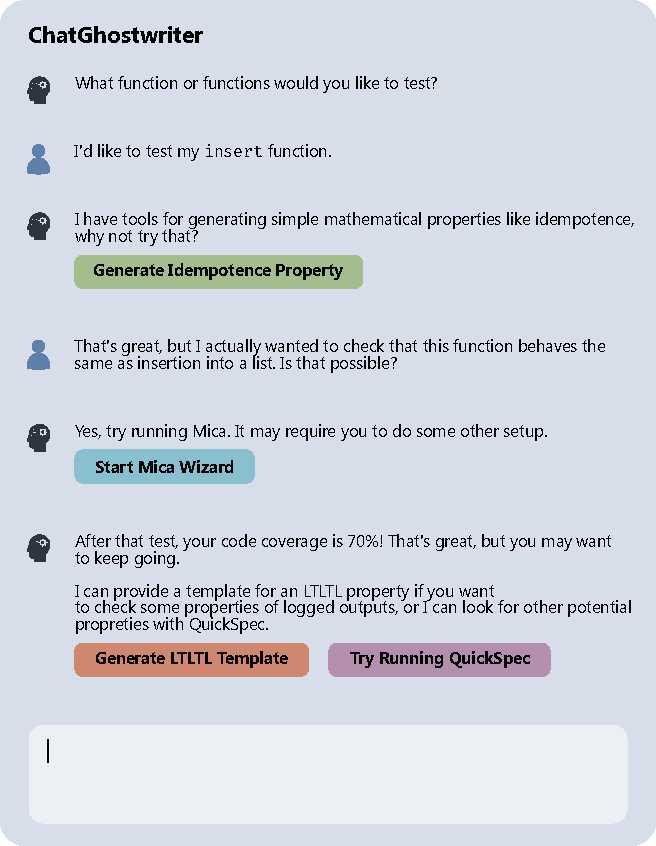
\includegraphics[width=.4\textwidth]{assets/chatghostwriter.pdf}
%   \caption{A mock-up of an interaction with \GhostChat. \bcp{Can
%       we make the text bigger and the whole thing smaller?  Or maybe
%       delete the whole thing in favor of Andrew's rewrite?}}
% \end{wrapfigure}
The above work will help us expand the settings in which PBT can be used with
great leverage.  That said, they do not yet address the problem that
testers---beginner and experienced alike---may face in writer's block
in figuring what properties to test in the first place (as our own prior work suggests~\cite{goldstein_problems_2022}). A complement of
programming assistant tools have recently come into wide use for situations just
like this. Perhaps most familiar are
Copilot~\cite{tool:copilot}, an in-editor AI that suggests one-liner completions and
function implementations which has seen widespread adoption among programmers~\cite{ref:dohmke2022github}; or ChatGPT~\cite{tool:chatgpt}, which in
myriad Twitter demos has shown its potential to take specifications in the
forms of text and sketches and through a chat-based dialogue generate nearly
fully-working implementations.

It is already possible for this technology to provide ideation
support for writing properties. Consider for instance one of the co-PIs'
conversations with ChatGPT about a module he had implemented in the
past~\cite{ref:chatgptpbtexample}.  In this conversation, the AI detects the data structures used,
and suggests a set of properties---e.g., data consistency, error handling, and
behavior in response to processing event sequences---and on further prompting suggests relevant
invariants to check following specific event sequences. The question is not
then whether modern programming assistants \emph{can} help with ideation of
properties, but how they might do it in a responsible way. \amh{I know
  I'm demonstrating the potential of ChatGPT in really unscientific
  ways---Twitter, prior experience---any better ideas?}  \bcp{How did
  we get to ``responsible''?}

We propose the development of integrated programming assistant features in the
editor that threads the needle of providing in-editor property ideation and
implementation support while relying on developer's cognition and trusted
property generation patterns wherever possible to ultimately lead to tests
that are both meaningfully and correct in all senses of the word. The envisioned
programming assistant would wrap existing property generation techniques---e.g., Mica
and LTLTL (proposed in the prior two sections), QuickSpec~\cite{ref:claessen2010quickspec}, and GhostWriter~\cite{ref:ghostwriter}---under APIs that allow them to be invoked
by an LLM programming assistant AI.

The envisioned interaction for a developer would be as follows. As a
developer writes code in their editor, analysis runs in the background to
identify those modules that are currently being tested by a large number of
input-output tests (and hence are likely worthwhile targets to ``battle test''
with PBT). Inline actions appear above the signature of those methods and the
functions that test them asking the developer if they would like to ``Test with
property?'' Upon clicking the action, the first step is for the AI to suggest
kinds of properties that may apply for this module (as was done in the example
cited above) and to recommend them as part of a simple list adjacent to the
code, e.g., ``You may wish to test this module's (1) round-trip consistency by
calling it and its reverse in sequence and its (2) resilience to null values in
arbitrary positions in the input sequence.'' This may be enough for developers
to overcome their writer's block. If it is not, the developer can further click
an action button to ``Generate tests.'' The programming assistant will
prioritize tests found by PL techniques (Mica, LTLTL, QuickSpec, GhostWriter)
due to their focus on existing high-leverage use cases and the guarantees they
provide about the correctness of generated code. Should they come up
empty-handed, the assistant will offer LLM-generated tests (as Copilot might
provide with suitable prompting) with the visible messaging conveying the
possibility of mistakes in the code or misinterpretations of user intent.

In this project, our work would be to prototype such programming assistant
functionality that integrates numerous components for property suggest,
and evaluate its support for overcoming the writer's block problem through
usability evaluations with developers.

PI Pierce recently began a collaboration with Professor Chris
Callison-Burch, an expert on computational linguistics and large
language models, who will work with us on this part of the project; a
letter of collaboration appears in the supplemental documents.

\amh{Needs more references}

\bcp{Sad that we lost the citation to TOGA.}

% \amh{Proposed workflow:
% The developer is working on testing a module.
% Their editor in the background checks for properties.
% It annotates the module (perhaps where it is invoked in a unit test) with an above-line marker reading ``Test with property?''
% The LLM generates suggestions of kinds of properties that could be tested---round-trip properties, invariants of the data structures, etc.
% It shows a small number of these suggestions in an overlay, and offers to create signatures with TODOs for those functions.
% Generated test signatures are then annotated with markers if their bodies can be generated for you.
% Generation is first performed by PL tools like Mica, QuickSpec, etc.
% If they cannot do it, the developer can request that the body of the test is generated by ChatGPT in a chat window, with a disclaimer about the uncertainty involved in the prediction.
% %
% This workflow is meant to balance prioritizing developers' agency in formulating their own properties, and leveraging existing tools for creating ``correct'' properties where LLMs might fall short, while still allowing developers to ``bottom out'' to asking an LLM for code generation in the event they still need help.
% }
% %
% High-leverage PBT scenarios provide a sort of recipe that developers
% can use to decide when and
% how to apply PBT, ensuring that they can get the most out of it.  But it is
% a shame that this recipe is only available to developers who have already
% internalized and understood it---ideally, a new developer with code that is
% easily PBT-able could jump into the process quickly and easily.  We propose
% embedding these high-leverage testing scenarios as automated tools and workflows
% in a programmer's editor.
% %
% Hypothesis currently provides {\em Ghostwriter}, a limited set of tools for
% automating the process of writing properties. It currently implements automatic
% property generation for round trip, equivalence, and other simple mathematical
% properties.  We would like to expand Ghostwriter to automatically infer
% properties in a much wider set of scenarios, via rich interactions with the
% user.
%
% Our re-imagining of Ghostwriter, dubbed {\em \GhostChat}, will be a chat
% interface that helps users to pick from a wide range of properties that might
% hold in their applications. The chat bot, inspired by successful large language
% model tools like ChatGPT~\cn{}, will be fine-tuned to analyze snippets of code
% and suggest property styles from a set menu that we provide. Once the user
% selects a property style, the extension will then run the appropriate
% classically-defined automation. This separation of concerns---a language model
% for the user interface, plus classical tools for actual property
% generation---maximizes both convenience for the user and correctness (since
% using a language model to produce properties directly may lead to subtle
% errors). \amh{If we propose the development of a new language model (or even a good language model) we probably need a letter of support from CCB / Dan Roth / Mark Yatskar, as neither I nor Benjamin have published prior work that will convince reviewers we are ready to do this. (I think we could do it, hahah, but I think we'll be seen as driving outside our lane.)}
%
% \GhostChat{} will be able to pull from all of the current Ghostwriter
% property types, as well as properties from Mica, LTLTL, and other tools from the
% literature like QuickSpec~\cite{ref:claessen2010quickspec}. Bringing these tools
% together with an interface that knows how to select between them and suggest
% configurations, will give users, especially beginners, a much simpler on-ramp to
% PBT. \amh{Why bother showing choices of property generators at all, if you can just generate them for the user without troubling them with choices? Maybe it's useful to tell someone about the kinds of properties that are getting generated and what they are meant to catch.} \amh{A more modern language model interface approach would be to have the LLM call each of the tools on the behalf of the user.} We will evaluate this tool with new users of PBT, evaluating their ability
% to get started from scratch.
%
% \amh{I think this is a lot closer. Though what this section is missing is a crisp definition of a key research insight that could merit a publication. (What takes this from cool demo to research paper?) Like, a specific way that the chatbot would teach people about the properties that are getting generated (if a more HCI contribution). Or, key insights about novel ways in which tools like QuickSpec, Mica, etc., would need to be tailored to interface with the LLM to support natural user queries or sensible LLM chat output.}
%
% \bcp{Also needs plenty of citations...}
%
% \bcp{Maybe this is a good application of Kani?}

\publicationtarget{IEEE Visual Languages and Human-Centric Computing (VL/HCC)}

% \SUBSECTION{Automatic explanations for properties}{sec:understanding}{4}{5}{HCI
%   Theory}{PhD 3}{REPL 7}{Pierce}
% Like any code, properties can
% be hard to understand, particularly by programmers who did not write
% them. Can we design
% tools to help explain them?

% We will explore how to design useful in-situ explanations of properties, for example
% explanations that could be viewed as just a few lines in
% tooltips and inline annotations in the editor and which clarify the meaning
% of an opaque property. This involves
% several research challenges.

% A first challenge is to simply address the right
% aspects of complexity; at the minimum, properties can
% be confusing because of their use of complex data (e.g., binary search trees,
% even logs), structural complexity (as is the cases for properties involving many
% predicates), or use of specialized syntax (as happens for advanced properties
% incorporating specialized operators in frameworks like QuickSpec). We know all
% of these manifest in some properties, but the frequencies are unclear.
% We will characterize complexity as it arises
% in the properties developers write by conducting a content
% analysis~\cite{ref:krippendorff2018content} of code bases using PBT.

% A second challenge is understanding how to generate explanations that will help
% a programmer understand properties at-a-glance. Several approaches may work well
% here.
% {\bf Input-Output Examples.} A first approach is to generate
% example input-output pairs demonstrating the behavior that a property tests.
% This approach is motivated by other recent efforts to generate input-output
% examples for instructional
% purposes (e.g.,~\cite{ref:gerdes2018understanding,ref:dantoni2015can}).
% We will leverage reflective generators and shrinkers to generate
% generating understandable inputs with potential complex structure, finding
% both positive examples and negative (i.e., failing) examples of program's behavior.
% {\bf Plain Language Explanations.} PI Head has prior work developing rule-based textual explainers of
% DSLs like CSS selectors and Unix commands~\cite{ref:head2015tutorons}; a similar
% approach might work in this context.
% The challenge in this research is understanding
% patterns of textual explanations that both ``speak the language'' of a reader,
% and which can be reliably generated from static analysis of the code.
% {\bf Large Language Models.} Large language models have recently
% made strides in being able to explain  source code; PI Head is
% exploring such technologies for general-purpose programming languages, and this
% approach may work well for frameworks like Hypothesis where properties are
% Python functions.

% The above efforts will contribute
% a characterization of complexity in property specifications,
% techniques for generating readable examples and descriptions for
% properties, and comparisons in
% usability studies.

% % \publicationtarget{PLATEAU Workshop}

\SECTION{Interaction}{PBT at Users' Fingertips
 \pagebudget{3}}{sec:val}

Our next thread of research focuses on developing powerful \emph{interactions} that afford developers new levels of visibility and control in PBT. The contribution will be novel techniques for evaluating testing effectiveness, and more direct mechanisms for developers to shape the distributions of generated inputs.

% and (3) understanding testing-provoked failures involving complex inputs
% (\sectionref{sec:failures})\bcp{same subsection!}.
%
% We also\bcp{where?} describe our plans to explore mixed-initiative
% interactions~\cite{ref:allen1999mixed}
% through which a developer can tailor a raw counterexample discovered by a
% PBT tool into source code for a maintaintable unit test
% (\sectionref{sec:counter}).
%
% \bcp{The last, especially,
% may read as ``Just engineering'' to some reviewers.  How do we clarify
% the research content there so that no one can miss it?  E.g., by emphasizing the
% investigate-needs/design/build/evaluate loop? I think addressing this
% point explicitly will help reassure (esp. non-HCI) reviewers.}
% \hg{Is the next paragraph not doing a good enough job here? We could move it
% up maybe?} \amh{Agreed, let me see what I can do.}

The projects in this thread
 will follow an
artifact-driven~\cite{ref:wobbrock2016research} HCI research methodology.
In this style of research, contributions come in several forms: insights into task
structure arising from close observational interviews, creation of novel
interaction primitives that map closely to these tasks, refinement of
technical methods (like those from \sectionref{sec:gen} and
\sectionref{sec:spec}) to support proof-of-concept implementations,
and distilling
lessons for interaction and algorithm design by evaluating these
implementations
with human users. Success will be measure by measured
reduction in
testing and debugging time and increased effectiveness.
PI Head has extensive experience with this style of work~\cite{ref:head2015tutorons,ref:suzuki2017tracediff,ref:head2017writing,ref:head2018when,ref:head2018interactive,ref:head2019managing,ref:head2020composing}.

\SUBSECTION{Tyche: An IDE for PBT}{sec:evaluating_distributions}{2}{3}{HCI
  Practice}{PhD 1}{REPL 8}{Head}
%
Our primary aim in this thread is the development of an integrated interactive toolkit to expedite the creation of good property-based tests. We focus our efforts on a particular aspect in PBT where interaction is the only way to improve current process: understanding and shaping input data distributions.

The effectiveness of PBT depends on the quality of input distributions, i.e., whether generated test cases are sufficiently ``interesting'' and sufficiently diverse.
% \todo{Cite the UIST demo -- proof of concept for feedback.  We will do
It is by no means easy for a developer to assess the quality of
an input distribution. A first challenge is simply understanding the shape of the distribution in the first place. Today, developers are limited to reasoning about the shapes of distributions on the basis of the description of the generator, or by creating custom visualizations. A second challenge is assessing whether the distribution is ``good,'' e.g., sufficiently representative of real-world inputs, likely to exercise bug-inducing paths in the software, etc.
A comon strategy for developers is to assess input distributions by inspecting a
small number of inputs. This process is slow, and necessarily leads to an incomplete picture of the distribution.
While HCI research has seen a renaissance of research in methods for visualizing input data distributions across myriad domains (e.g.,
~\cite{ref:hohman2019gamut,ref:hohman2020understanding,ref:kang2017omnicode}), new solutions are needed for PBT.

What about the PBT setting requires novel solutions?
In PBT, test inputs are
programmatically generated and
can be of unbounded structural
complexity (e.g., lists, trees, other algebraic data types,
sequences of API calls).
For example, a developer might want to generate
realistic logs of input data, where each log entry includes at least a timestamp
and an event type.
%
Ideally, the developer would be able, by examining the generator's
distribution, to answer
questions like: Are the generated log inputs long enough? And are most
of the event sequences realistic?
Our research will contribute the interaction primitives and
 unifying environments necessary to answer questions like these.

%
\begin{wrapfigure}{r}{0.58\textwidth}
  \centering
  \vspace*{-2ex}
  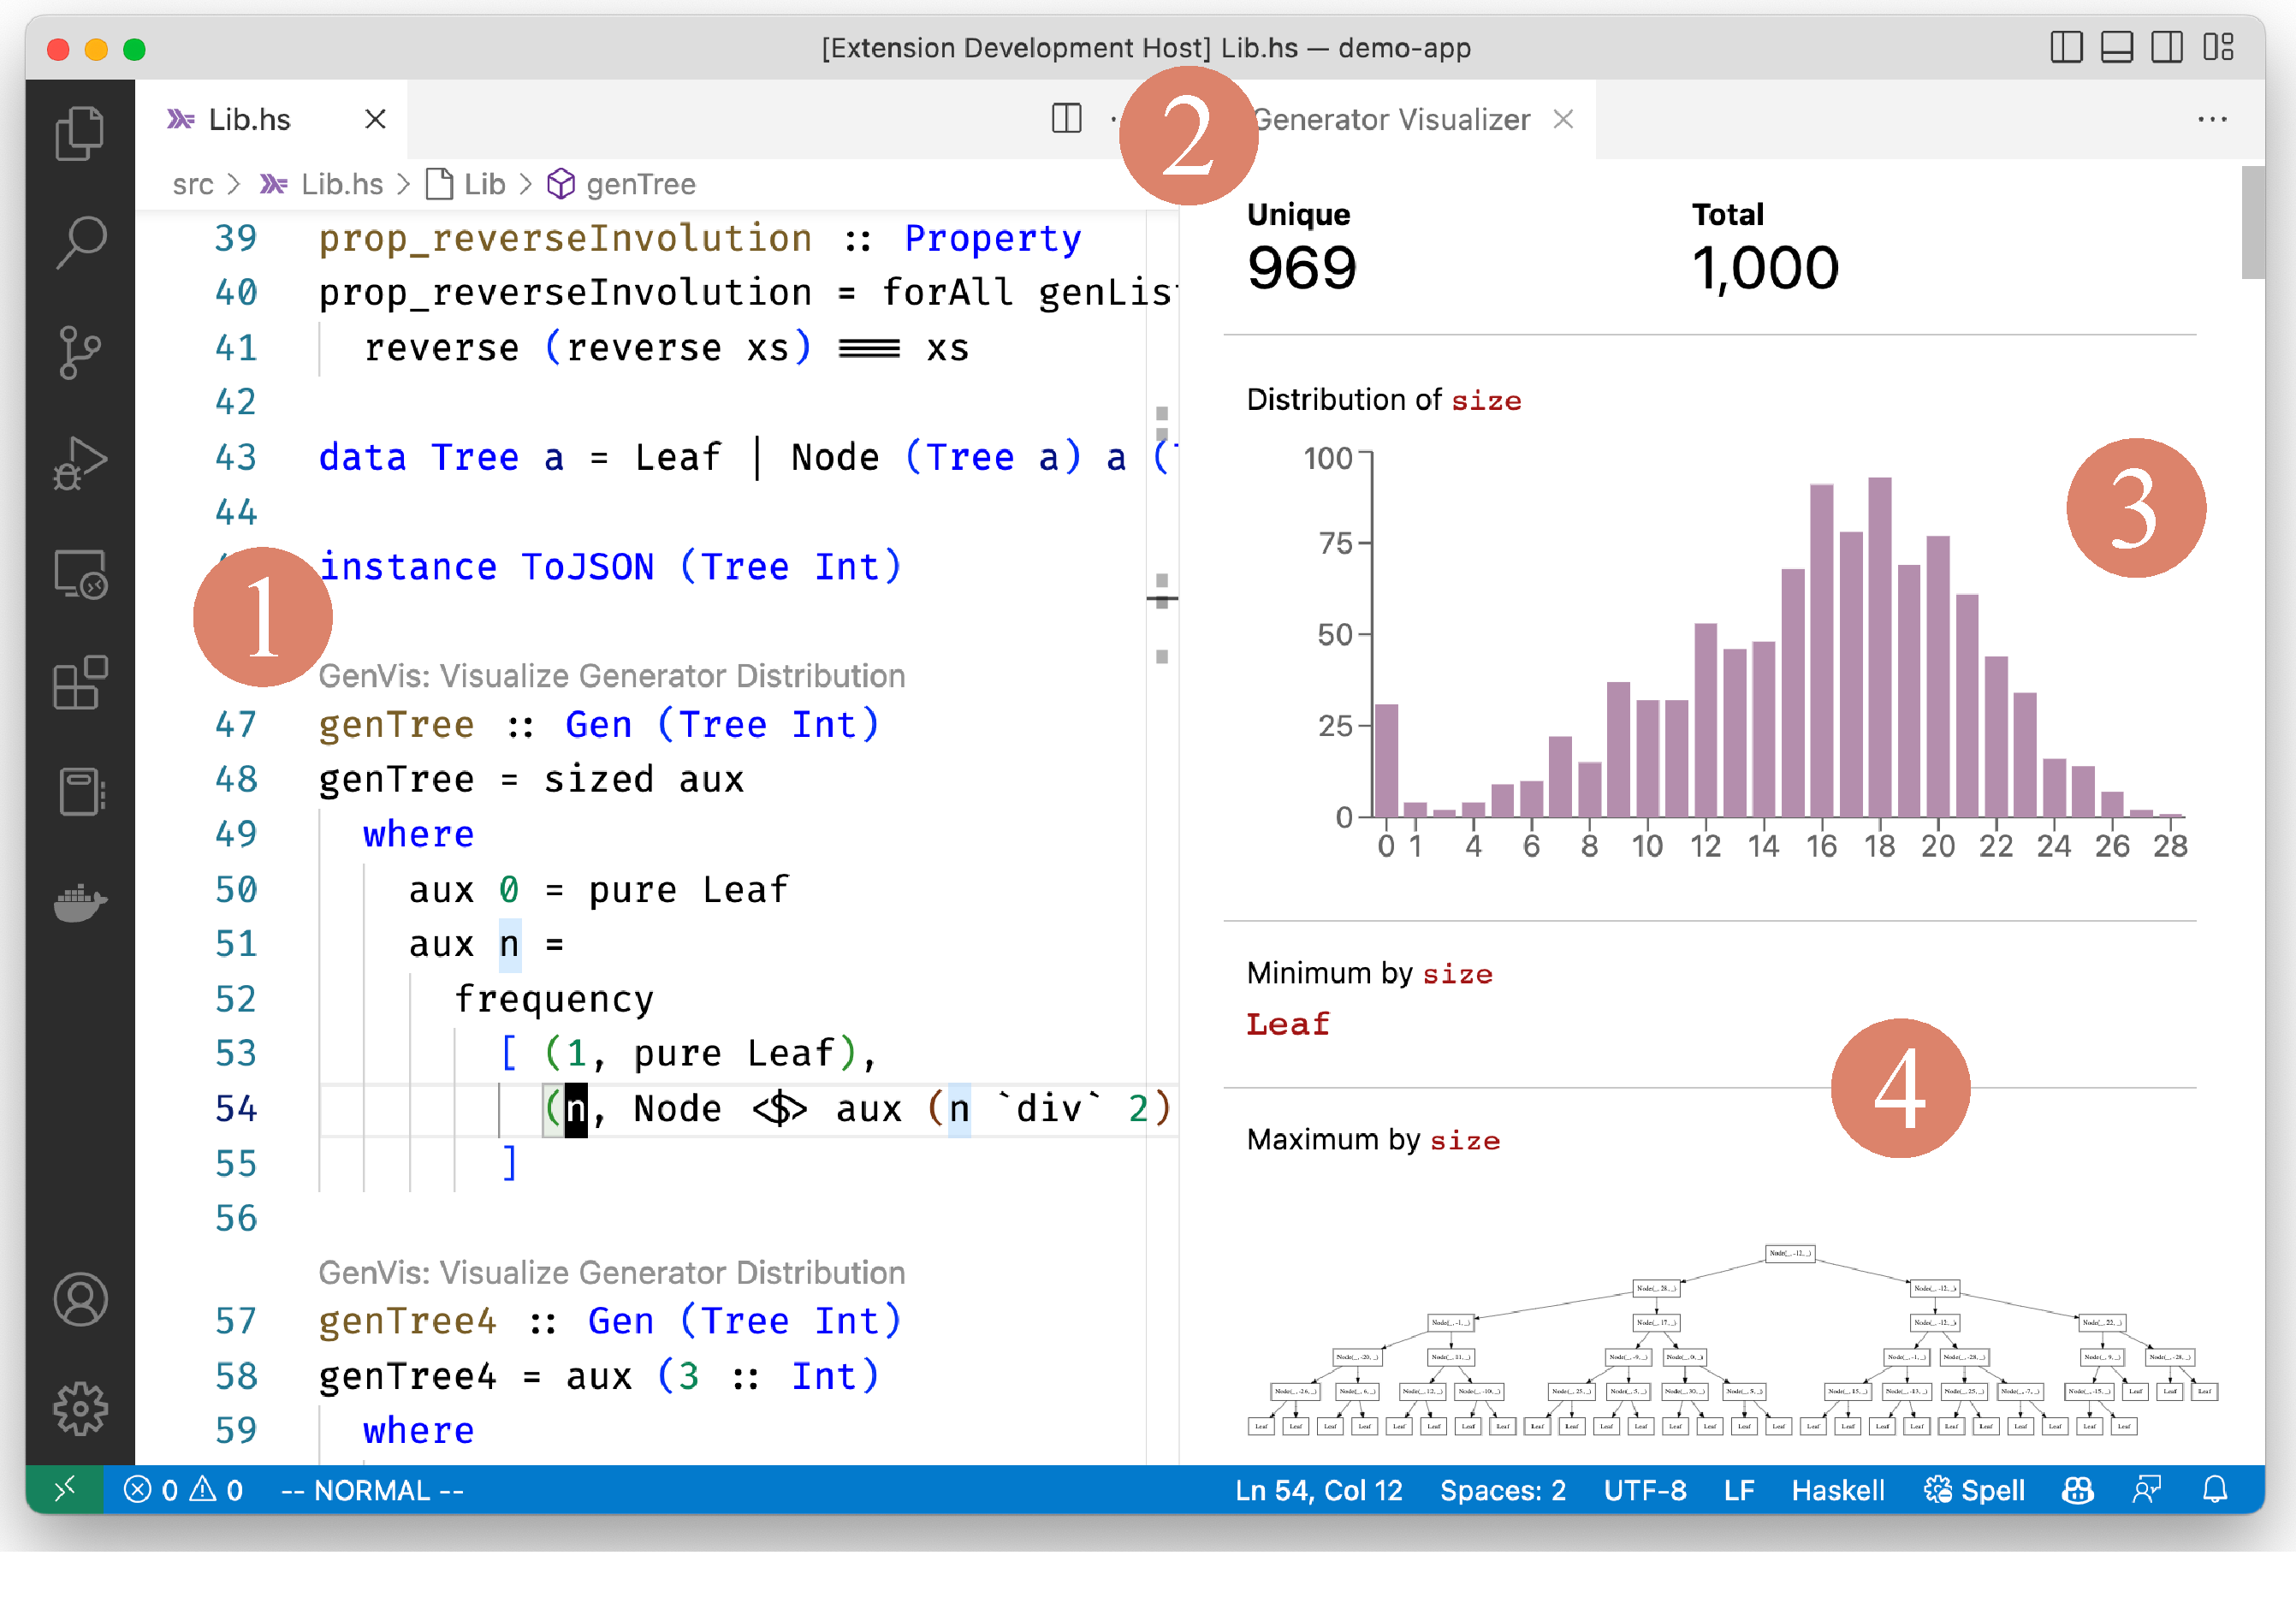
\includegraphics[width=0.58\textwidth]{assets/gen-vis.pdf}
  \caption{A tool for evaluating data distributions, showing
  generator source code (1), summary statistics (2),
  aggregate visualizations (3), and views of input instances
  (4). Iteration would be supported with live adjustment of
  generator code and refinement of filters used in the
  visualizations.}\label{fig:gen-vis}
\end{wrapfigure}
%
 {\subsectionstar{An interactive toolkit for PBT}{}{} %
 We will develop an interactive toolkit that provides integrated
 support for understanding and tuning data distributions.
We call this toolkit \tyche{}, after the Greek goddess of
chance. Below, we describe the major affordances we envision
developing through the program of research. We will develop \tyche{}
as an extension to Visual Code, a modern editor that sees widespread
adoption~\cite{noauthor_stack_nodate} and support for every language
with mature PBT tooling. We plan for \tyche{} to serve as a platform
for developing not just those interactive features describe here, but
by other groups. A prototype of \tyche{} has been built and has been
accepted for the UIST demos session~\cite{ref:goldstein2023tyche}; a
mockup appears in Figure~\ref{fig:gen-vis}. The novel features that we
will develop in our research follow:

\subsectionstar{Understanding Input Distributions}{}{}
The first research innovation will be the design of live displays of generated
values. These displays
will show aggregate data views, including aggregate
statistics (Figure~\ref{fig:gen-vis}.2) and visualizations of the distribution
of important summary features of the data (Figure~\ref{fig:gen-vis}.3). The
displays will be live~\cite{ref:tanimoto1990viva} and real-time. Noting the
success of other successful live functional programming environments in industry
and academia
(e.g.,~\cite{tool:lighttable,ref:omar2019live}), we anticipate liveness will
provide visibility and control (i.e., the ability to change or halt)
long-running, opaque data generation processes.  Visualizations will be
generated using recommendation rules as done in related work in exploratory data
analysis~\cite{ref:lee2021lux,wongsuphasawat_voyager_2016,
wongsuphasawat_voyager_2017}. Unique to our setting, the tool will leverage
type-based automation and user-defined functions to extract features to
visualize.
For example, consider the
\lstinline{log} type
from above. A developer might be interested in the log's
\lstinline{length}, field accessors like \lstinline{event_type}, \lstinline{id},
and \lstinline{timestamp}, filters like \lstinline{is_empty}, and
aggregators like \lstinline{max_by}. Such features can be
generated automatically for common data types.
% Then the tool will then use
% lightweight type-based program synthesis to compose and combine these functions
% to get features. It may choose to show the \lstinline{length} of a log, but also
% the \lstinline{max_by (fun l -> length l.payload)} (the maximum payload length),
% and even pairs of features like these (which could be viewed as a two
% dimensional feature).

A second innovation will be environmental support for rapid customization with
user-defined functions.  If
there are features that the developer notices should be extracted but that the
system cannot come up with itself (e.g., \lstinline{ids_unique}), the developer
can
write them alongside their property specifications;
the interface will automatically load those features into the
display.

A third innovation will be interaction primitives for drilling down into
individual inputs from aggregate views by selecting marks in visualizations
(e.g., choosing a bar
of length ``10'' to preview individual inputs with that length). Prior HCI tools
(e.g.,~\cite{ref:hohman2019gamut})
provide this feature generally. What is unique in our domain is to provide
suitable representations of complex inputs that
will be easy to understand. Some general solutions might be to
pretty-print inputs, provide interactive object browsers like those available
in JetBrains~\cite{tool:jetbrains}, to allow a developer to explore an
object using a built-in REPL, and to produce
DOT~\cite{ellson_graphviz_2002} representations of common kinds of
inputs (i.e., lists, trees) for at-a-glance comprehension of
larger inputs (Figure~\ref{fig:gen-vis}.4). We will try each of these
approaches and compare their effectiveness in pilot studies.

A fourth innovation is the synchronization of above views with
live feedback on what code is exercised by the tests. Building on the design
pattern whereby a tool show which lines of code are currently
executing~\cite{ref:brandt2010rehearse,
  ref:oney2009firecrystal, ref:burg2013record}, our tools will
colorize code to show
how frequently each line is executed while running tests, both in aggregate and
for individual tests. Altogether, the above activities will be a set of
interrelated interaction primitives that serve as building blocks for
understanding distributions of complex input data. Success of this (and the next
two projects) will be determined by the novel interactions' ability to reduce
testing time and achieve desirable input distributions.

\publicationtarget{User Interface Software and Technology (UIST)}

\subsectionstar{Interactive Tuning of Input Distributions}{}{}
%
Tuning generators to produce ``interesting''
values can be challenging, requiring
significant trial and error with a generator description.
% Automated approaches like reflective generators (see \sectionref{sec:generation}) Purely automated approaches
% such as those involving reflective generators (\sectionref{sec:reflective}) provide part of the
% solution, as do code coverage-based generation techniques
% (e.g.~\cite{afl-readme}). That said,
% even these techniques fall short of the kinds of inputs a developer would wish
% to produce.
We will develop new methods for specifying desired distributions through interaction. One innovation we
will work on is to support tuning by manipulating the visualizations described in the previous section. The goal is to enable a kind of
bidirectionality for PBT programming that has seen success in other areas of
programming research (e.g.,~\cite{ref:hempel2019sketch, ref:kery2020mage,
  ref:omar2012active, ref:omar2021filling}).
 A first approach is via input filtering: a developer could
select a region (e.g., a bar) in an aggregate visualization and request that
inputs from that region are discarded before testing. This approach is flexible
but limited, as it does not change the underlying generator.
% It may also lead to inefficiency, if too many values are
% generated from the distribution only to be discarded by the
% filter.

Therefore, we will design additional interactions that leverage the unique
ability of reflective generators developed in this project
(see \sectionref{sec:gen}) to change the underlying
generator parameters. As developers interact with a visualization,
the reflective generator will map interactions (e.g., altering the height of a bar)
to choices
in the generator (e.g., indicate a preference for the kinds of inputs represented by that bar).  The generator code will be displayed
side-by-side with visualizations of the distribution, and the user
will be able to manipulate both sides.
Developers will be able to interact directly with the visualization to
indicate, for example, that they would like to see more inputs like
one that has already
been generated, or that they would like an input similar to a generated input,
but different in a way that they are demonstrating.

% This project and that in
% \sectionref{sec:evaluating_distributions} will together yield new paradigms for
% understanding and changing input data distributions.

\publicationtarget{User Interface Software and Technology (UIST)}

\iflater
\amh{I removed the goal of 60k downloads (it's now in the comments). It felt a bit over-ambitious without a staff engineer and 5 years of work.}
% We will make \tyche{} known to the developer community through talks at developer
% conferences and by
% disseminating information via our contacts in industry and the open source
% community.
% %
% % We will list the IDE on the Visual Studio Code extension marketplace,
% % with a goal of reaching 60,000 downloads by the end of the project.
% Our goal is for \tyche{} to reach 60,000 downloads by the end of the
% project. At
% the time of writing, this would put \tyche{} in the top 10 extensions
% tagged ``Testing'' in the Visual Studio Code extension marketplace
% that are not either full language servers or Large
% Language Model interfaces~\cite{noauthor_testing_nodate}.

% We aim for \tyche{} to reach 60,000 downloads by the end of the
% project, driven, in part, by our connections in the developer tool community.

\amh{If we don't have enough content for this proposal, it might be worth adding back in 1--2 paragraphs of our strongest material about interactive shrinkers.}
\amh{Or, maybe better yet, the work on creating regression tests from counterexamples, which could be a good project for a REPL student.}
\fi

\proposecut{
\SUBSECTION{Interactive shrinking and
  debugging}{sec:failures}{3}{3}{HCI Practice}{PhD 1}{PhD 2}{Head}
\bcp{I wonder whether this whole subsection could be eliminated or
  reduced to a paragraph in a longer discussion of possible extensions
  of Tyche -- it seems weaker than most of the rest...}
%
As with any kind of testing, one challenge with PBT is understanding why
a given counterexample triggers a failure. We will explore new interactions that
take advantage of the machinery available from PBT tooling to help programmers
understand failures.

Our first effort will be to design interactive input shrinkers. Typical
automated shrinking approaches
(e.g.,~\cite{hughes_quickcheck_2007,arts_shrinking_2014}, and our own
proposed techniques
in \sectionref{sec:reflective}) can get stuck at local minima far from the
global minimum, without realistic ways for users to get them unstuck. But
developers can see shrinking options that a shrinker may not.  Could
interaction help a developer shrink a stubbornly large input?

We can take inspiration here from HCI research on incremental code simplification
(e.g.,~\cite{ref:lim2018ply,ref:head2018interactive,ref:holmes2012systematizing,ref:hibschman2016telescope}),
but new ideas are needed when the simplification target
is code with recursion and/or complex data. We propose a semi-automatic
interaction paradigm where a developer performs some simplifications
manually in an interactive
object viewer (like those in modern debuggers like JetBrains
IDE~\cite{tool:jetbrains}) while a shrinker attempts further
simplifications in the background. The system would
display
the valid ways an input can be altered,
determined using reflective generators,
and
automatically
shrink after each action.

We also see opportunities to help developers find the root causes of
failures in a PBT setting. A current approach is implemented by Hypothesis'
\texttt{explain} module, which points users to lines that are always run during
failed tests but never during successful tests. But we
found this technique to be inconsistent\bcp{meaning it didn't work
  consistently? or we couldn't consistently understand what it was
  telling us? or...?}, even on examples provided in the
Hypothesis documentation.
Could a tool highlight divergences in more useful ways?

A prior project involving PI
Head designed views of trace divergences for student
programmers debugging failed submissions versus a reference
program~\cite{ref:suzuki2017tracediff}, but this technique is not
quite right for
PBT, where is no correct program to compare to.  Instead,
we need to show divergences in a way that (1) points programmers to control
decisions that vary between a failure-inducing input and a set of very similar
success-inducing ones (using the reflective generator framework to assess
similarity); (2) shows what lines will be executed next following the control
decision by the gamut of comparison inputs\bcp{??}; and (3) supports rapid
navigation between
control decisions in the case of greatly diverging traces. We will iteratively
design, implement, and evaluate a tool supporting such interactions.
\bcp{All that could use an example.}

\publicationtarget{User Interface Software and Technology (UIST)}
}

% \publicationtarget{Foundations of Software Engineering (FSE)}

\SECTION{Diffusion}{Impact on PBT in Practice}{sec:diffusion}
% \SECTION{Diffusion}{Advancing Open-Source Tools}{sec:diffusion}

The foundational research and tool building projects described above
are needed, we believe, to bring PBT to a broader audience,
but they not enough by themselves. Our agenda also
includes plans for increasing the {\em diffusion} of PBT by developing the Tyche IDE as a
cross-platform, language-agnostic, open-source project (\sectionref{sec:ide}), educating
programmers in effective application of PBT by developing a catalog of
high-leverage PBT use cases (\sectionref{sec:whento}), and
creating undergraduate- and
master's-level course materials for PBT (\sectionref{sec:1210}).
We will also advertise our findings, tools, and materials to potential user communities
through talks at industry conferences like Yow! Lambda Jam, Strangeloop, and
Lambda World.

\SUBSECTION{An Open-Source Community around Tyche}{sec:ide}{2}{3}{Tech
Transfer}{???}{}{Pierce}
The Tyche IDE will be developed in consultation with
our collaborators on the Hypothesis team (see Collaboration Plan) to
enable tight integration with existing features of modern PBT systems,
facilitate future adoption, and develop opportunities for long-term maintenance
by the open source community.  We are also in discussions with
leadership at Amazon AWS, who are interested in devoting engineering
resources to developing a version of Tyche for Rust programmers.
We will foster external contributions by developing Tyche as a
public,
open-source project and creating appropriate technical and
social mechanisms for external collaboration.
%
% \proposecut{We will also advertise \tyche{} to potential user communities through talks at developer
% conferences and by
% disseminating information via our contacts in industry and the open source
% community}.
% %
% \proposecut{%
% The research projects described above have the potential to
% dramatically improve the power and usability of PBT, but only
% if their products are attractive to real users. There is an unfortunate tendency for
% research software to remain just that---missing critical
% documentation that new users need to get started and lacking a clear
% maintenance schedule that would give software companies the confidence
% to adopt.
% To avoid this fate for our projects, the PhD students will work closely with our
% research engineer. The code for those projects will be designed with learnability and
% maintainability in mind, and upon
% completion it will be handed off to appropriate owners
% in the open source community.
% }

% Old Tyche text below
% The projects in \sectionref{sec:val} will explore a wealth of new modes of interaction
% for PBT. Their potential impact will be magnified by
% integrated them into a system
% that is attractive to would-be users. This is the inspiration for
% \tyche{}, an IDE extension for PBT.
% \tyche{} will first serve as a platform for building and testing all the functionality designed in \sectionref{sec:val}. Promising features from research will constitute its core.
% \tyche{} will be developed as a Visual Studio Code extension, taking advantage
% of VSCode's status as the most widely used editor according to a 2022
% survey~\cite{noauthor_stack_nodate} and its support for every language
% with mature PBT tooling.

% To maintain focus, we will concentrate our Efforts on making \tyche{} especially effective for one
% widely used
% PBT framework---probably Hypothesis, since
% its developers
% have expressed interest in including
% \tyche{} in the main Python language extension for VSCode.
% But we will make the code of \tyche{} language-agnostic wherever
% possible, to allow other
% language communities to use it with their PBT frameworks.

% The research engineer will lead feature integration, ensuring features come together into a
% seamless whole. They will also develop \tyche{} to serve as a platform for
% further innovation as it will have been for our own: extension points will be added
% for others to create and evaluate techniques for understanding and creating properties and generators.
% In this way, \tyche{} will provide a pipeline for bringing research on
% PBT algorithms and interaction models to developers craving better tools.

% We will make \tyche{} known to the developer community through talks at developer
% conferences and by
% disseminating information via our contacts in industry and the open source
% community.
% Our goal is for \tyche{} to reach 60,000 downloads by the end of the
% project. At
% the time of writing, this would put \tyche{} in the top 10 extensions
% tagged ``Testing'' in the Visual Studio Code extension marketplace
% that are not either full language servers or Large
% Language Model interfaces~\cite{noauthor_testing_nodate}.


% \SUBSECTION{Nurturing the PBT ecosystem}{sec:nurturing}{1}{5}{Tech
% Transfer}{Engineer}{PhD 1}{Pierce}
% The existing ecosystem of open-source PBT tooling is broad and varied. Some
% projects are vibrant, while others, including some with
% great ideas and implementations, do not have the developer bandwidth to address
% user needs. Additionally, existing frameworks have not been designed with
% the benefit of the insights and tools that we will build in this
% project, leaving (we believe) large opportunities for improvement.
% Thus, we will allocate a significant part of the engineer's time to
% supporting and improving open-source PBT frameworks.
% %
% To make best use of limited resources, we will choose existing PBT
% frameworks as targets and use the findings and software products from
% our research to boost their usability and adoption.
% % \amh{This sounds like a lot. I'd strongly advocate for just 1 and doing it really well, given that serious involvement in an open source project can be a full-time job, especially if it requires careful coordination with the project's team and evolution of its core code base. I think the claim that we're offering to maintain 3 open source projects and produce an extension of our own and support research will probably raise a red flag for those concerning themselves with engineering logistics.}
% % \amh{If we really want to stick with 3 projects, I think we should commit to maintaining at most 1 open source project, and for the other 2 projects just integrate novel features.}

% We will start
% with Python's Hypothesis framework, since it is well-established and yet has
% significant room for growth.  We are in contact with Zac Hatfield-Dodds, the
% main maintainer; a letter of collaboration from Mr.{}
% Hatfield-Dodds appears in the supplemental documents. The Hypothesis team is
% especially excited about integrating ideas like reflective generators
% (\sectionref{sec:reflective}) and interaction modes like distribution
% visualization (\sectionref{fig:gen-vis}) into Python's VSCode environment.
% The success of this collaboration will be measured by the Hypothesis team's
% willingness to include our tools in future releases and by uptake in the community.

% Besides Hypothesis, we will choose two additional projects to contribute
% to in smaller ways, prioritizing great
% projects in popular programming languages that have significant room
% for growth. Candidates include
% Scala's ScalaCheck,
% OCaml's Crowbar, which has great ideas and
% some attractive low-hanging fruit~\cite{noauthor_shrinking_nodate}, and projects like
% \lstinline{jqwik} in Java or \lstinline{proptest} in Rust, which are
% embedded in massive language
% communities that could benefit from better tools for PBT.
% We will work closely with the
% developers and maintainers of these projects to ensure that our input
% is well received by the community.

\SUBSECTION{``When to Specify
  It!''}{sec:whento}{1}{1}{Education}{Faculty}{Everyone else}{}
%
% Another way in which we plan to disseminate PBT is through creating new
% educational materials.
Our interviews with industry developers suggest that many
have a tacit
understanding of several ``no-brainer'' situations where PBT is a natural
choice---where properties are easy to find and PBT provides
more thorough testing than other techniques---and
seem happy to limit their use of PBT to such situations.
While more experienced PBT users do also apply it in less obvious,
high-cost / high-benefit situations, it appears that
focusing educational efforts on easy cases may be the best way to
drive adoption.

We plan to produce educational resources to help developers understand
high-leverage situations for PBT. We will begin with an effort
tailored to the academic community: a survey paper with the
aspirational title ``When to Specify It!'' in homage to John Hughes's
popular tutorial, ``How to Specify It!''. Initially,
the survey will
document a  range of high-leverage scenarios identified by our formative
industry study%
.%
\proposecut{, including cases like
\begin{enumerate*}[label=(\arabic{enumi})]
\item ``these two functions (e.g., a parser and a printer) should round-trip,''
\item ``this data structure (e.g. a set, map, etc.) should obey algebraic laws,''
\item ``this stateful module should uphold an invariant,''
\item ``these two programs should behave the same'' (e.g., because one
is an optimized version of the other),
and
\item ``this program should not crash.''
\end{enumerate*}
}
As the project progresses, this list will be expanded based on
further surveys with broader
communities of developers~(\sectionref{sec:survey}), a comprehensive
review of case studies in
the academic literature, and an examination of open source projects
using PBT in a
variety of different software ecosystems.

\SUBSECTION{Curricula for PBT}{sec:1210}{1}{3}{Education}{Faculty}{Engineer}{}
%
University education can act as a force
multiplier to drive adoption of new
technologies in industry.
We will develop materials for
integrating PBT into early undergraduate and masters-level courses. As
noted in \sectionref{sec:whento}, testing well-defined data
abstractions is one of the high-leverage scenarios for using PBT.
%
Concretely, building on
recent explorations of PBT teaching in data structures
courses~\cite{wrenn2021using, nelson2021automated}, we will integrate PBT into
Penn's second-semester CIS 1200 course, which PI Pierce regularly teaches.
%
We
will evolve the CIS 1200 curriculum to emphasize themes in PBT from our
formative research---good circumstances for
using PBT, methods for writing useful generators, properties as
documentation, and scenarios where PBT is especially suitable
(see~\sectionref{sec:whento}).
%
We will also include PBT in Penn's CIS 5730, a masters-level software
engineering course.
%
We will evaluate the impact of these new
instructional approaches on students' ability to leverage PBT in final
projects.
%
Our instructional materials will also be made available for
instructors at other institutions.

\publicationtarget{SIGCSE or Koli Calling International Conference on
  Computing Education Research}

\immediate\closeout\workplanfile
% \SIMPLESECTION{Plan of Work\pagebudget{.7}}{sec:plan-of-work}

% \bcp{I've moved the text that was here to a separate supplemental
%   document, but we'll probably want to say something short in the main
%   project description (either here or, better, toward the top) about
%   synergy and coordination, with a pointer to that document.}

% \begin{figure}[ht]
%   \centering
%   \vspace*{-1in}
%   \hspace*{-.4in}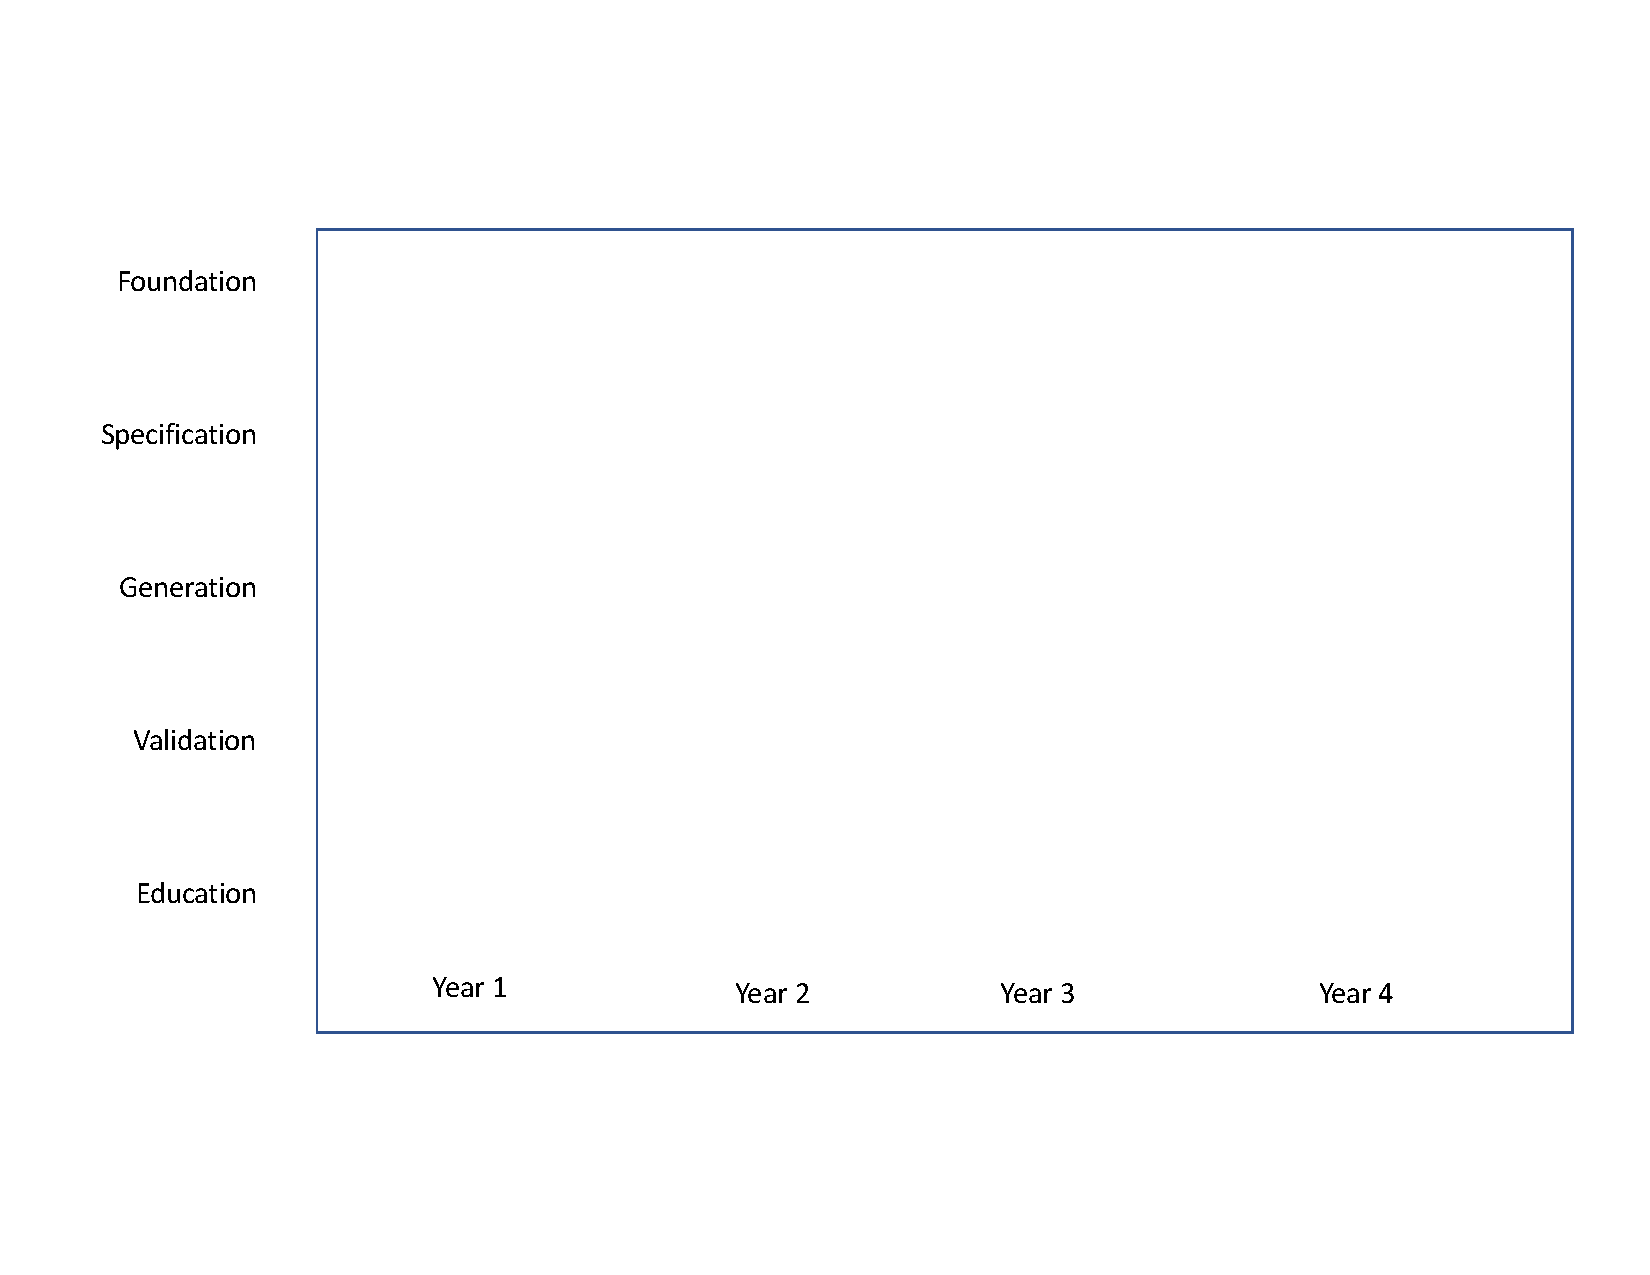
\includegraphics[width=1.1\textwidth]{assets/workplan.pdf}
%   \vspace*{-1.3in}
%   \caption{Plan of work.}\label{fig:workplan}
% \end{figure}

% \vspace*{-.4in}


\SIMPLESECTION{Broader Impacts%
 \pagebudget{.5}}{sec:broader-impacts}

Broad impact is key to our research agenda, and many of the concrete
tasks we have described---particularly those grouped under Diffusion
(\sectionref{sec:diffusion})---are specifically aimed at broad
impacts.  Here, we summarize those aims and sketch our plans for
mentoring, diversity, and broadening participation in computing.

\smallskip
\noindent{\bf Impact on industry.} The main broad impact from the
proposed work will be a significant increase in the use of PBT across
the software industry within the time frame of the grant, driven
by more powerful and usable tools, driven principally by open-source
tools (\sectionref{sec:ide}).
\bcp{How will we measure success?}

\smallskip
\noindent{\bf Impact on Education.}
%
A second, supporting arena for broad impact will be the
development of educational materials for both students and
professional developers. Educational activities will be
coordinated with the rest of the work and are integral to the
project's overall goal of making PBT a standard testing methodology.
Specific pedagogical
threads within the project are described in \sectionref{sec:whento} and \sectionref{sec:1210}, but the
tasks in \sectionref{sec:foundation}, \sectionref{sec:reflectiveusable},
\sectionref{sec:interactive}, \sectionref{sec:understanding}, and
\sectionref{sec:evaluating_distributions}\bcp{fix} will also influence education. The
work in \sectionref{sec:1210} will generate course materials that we will
share publicly, and we will share our experiences in a paper at a
CS-Ed-focused conference.

An ancillary educational goal is to
publicize and communicate the benefits of PBT to the broader computer science
{\em research} community. As part of these efforts, we will write an article on PBT
for the Communications of the Association for Computing Machinery
(CACM).

\smallskip
\noindent{\bf Mentoring and Diversity.}
%
The majority of the requested funding will support formative research
experiences and mentoring for graduate students. Each graduate
student will lead multiple facets of the
project, including co-supervising undergraduate
researchers.
%
The PIs will recruit graduate students for this project with a mind towards making
the research area reflective of diversity in the US and Pennsylvania.
The PIs have already made inroads broadening participation of women in their
groups (1/3 of Pierce's current PhD students and 2/4 of PI
Head's are women).

A particular focus
will be increasing representation of
other underrepresented groups, including Black and Latinx
students. Pierce (along with Penn colleagues Zdancewic and Weirich)
recently received funding for an
NSF REU program that will involve 24 undergraduates (either per
year for three+ years), selected specifically with an eye to diversity;
for the present project, we are requesting funds to add one more per
year specifically to work on PBT topics, many of which are well suited
to undergraduate interns. See the BPC
supplementary
document for more details.

\smallskip
\noindent{\bf Benefits to Society.}
%
The project's goals will also be advanced by open-source distribution of tools
built during the project, in particular Tyche
(\sectionref{sec:evaluating_distributions} and
\sectionref{sec:ide}). These will be distributed under a permissive
open source license to serve as models for similar tools in other
programming languages and environments.

This project also presents excellent opportunities for strengthening
collaborations between university researchers and industrial advocates
of PBT.  Our preliminary industry study was carried out with the
enthusiastic support of Jane Street's developers and management, and we plan
to use Jane Street as a testbed for prototypes of our
tools.  We are also collaborating with the
developers of Hypothesis, who are keenly
interested in the results of this proposal, and we are in early
discussions with technical leadership at AWS about potential
collaboration on Tyche.  \proposecut{We hope to establish connections with the
developers and user communities of popular PBT tools in languages like
Java, Rust, and Scala.}

In the long term, better testing means better software.  As software
systems have grown to the gigantic scales seen today, good testing
methodologies and tools---unit testing tools, test-first design
methods, etc.---have come to play an ever more crucial role.  Adding a
powerful new testing tool to programmers' toolbelts will further streamline
this aspect of the development process, leading to software of every
sort that is more robust, more reliable, and less expensive. \bcp{If
  we've talked about the need to vet LLM-generated code earlier in the
  proposal, we need to reiterate it here.}


% \proposecut{See the Collaboration Plan for
% more.}

% The Project Description must contain, as a separate section within the narrative, a section labeled ``Broader
% Impacts of the Proposed Work". This section should provide a discussion of the broader impacts of the proposed
% activities. Broader impacts may be accomplished through the research itself, through the activities that are
% directly related to specific research projects, or through activities that are supported by, but are complementary to
% the project. NSF values the advancement of scientific knowledge and activities that contribute to the
% achievement of societally relevant outcomes. Such outcomes include, but are not limited to: full
% participation of women, persons with disabilities, and underrepresented minorities in science, technology, engineering, and
% mathematics (STEM); improved STEM education and educator development at any level; increased public
% scientific literacy and public engagement with science and technology; improved well-being of individuals in
% society; development of a diverse,globally competitive STEM workforce; increased partnerships between
% academia, industry, and others; improved national security; increased economic competitiveness of the United
% States; and enhanced infrastructure for research and education.

\SIMPLESECTION{Results from Prior NSF Support\pagebudget{.5}}{sec:prior}

\todo{Double check conformance with GPG rules: The following
  information must be provided:
(a) the NSF award number, amount and period of support;
(b) the title of the project;
(c) a summary of the results of the completed work, including accomplishments, supported by the award. The results must be separately described under two distinct headings: Intellectual Merit and Broader Impacts;
(d) a listing of the publications resulting from the NSF award (a complete bibliographic citation for each publication must be provided either in this section or in the References Cited section of the proposal); if none, state “No publications were produced under this award.”
(e) evidence of research products and their availability, including, but not limited to: data, publications, samples, physical collections, software, and models, as described in any Data Management Plan.}

% If any PI or co-PI identified on the project has received NSF funding (including any current
% funding) in the past five years, in formation on the award(s) is required,
% irrespective of whether the support was directly related to the proposal or not.
% In cases where the PI or co-PI has received more than one award (excluding amendments),
% they need only report on the one award most closely related to the proposal. Funding includes not just salary
% support, but any funding awarded by NSF. The following information must be provided:\\

\emph{\underline{PI Pierce}}: ``Collaborative Research:
SHF: Medium: Bringing Python Up to Speed'' (NSF 1955565, \$1,200,000
[Pierce's share: \$437,999],
7/2020--6/2023), with co-PIs Michael Hicks (U. Maryland) and Emery Berger
(U. Mass Amherst).
The project aimed to dramatically increase the performance and
correctness of applications written in Python by developing novel
techniques for performance analysis, optimization, run-time systems,
property-based random testing, concolic execution, and program
synthesis. It developed both
novel performance analysis tools and optimizations and novel automatic
testing frameworks. These were largely tailored to and implemented for
Python, but applicable in other, similar languages.
%
{\bf Intellectual Merit.} The project involved work on both
performance measurement (mostly at Amherst and Maryland) and PBT (mostly at Penn
and Maryland).  Specific threads of work involving Penn included
building an early
version~\cite{Frohlich2023} of the Reflective Generators described in
\sectionref{sec:gen}, carrying out the pilot study of PBT in Python
mentioned in
\sectionref{sec:motivation}~\cite{goldstein_problems_2022},
building on the idea of
freer monads from functional programming to develop ``free
generators,'' which unify parsing and
generation~\cite{goldstein2022parsing},
presenting a principled
automatic testing framework for application-layer
protocols~\cite{Li2021:MBToNA}, and developing and releasing a freely
available mutation testing framework for Python, called {\tt
  pytest-mutagen}~\cite{pytestmutagen}, and applied ideas from
combinatorial testing, a widely studied testing methodology, to modify
the distributions of random test-case generators so as to find bugs
with fewer tests~\cite{DBLP:conf/esop/GoldsteinHLP21}.
%
{\bf Broader Impacts.} Project results and open-source software
products are being used to increase the
performance and correctness of Python applications.
Educational impact focused on training graduate and
undergraduate students, including a female PhD student, Jessica
Shi.
%
{\bf Publications (involving Penn):} \cite{Frohlich2023,DBLP:conf/esop/GoldsteinHLP21,
  goldstein2022parsing, goldstein_problems_2022, Li2021:MBToNA}.
{\bf Research Products (involving Penn):} \cite{pytestmutagen}.

\smallskip

\noindent\emph{\underline{PI Head}} has not previously received NSF support.

% \SUBSECTION{Proposed Study}{}{}
% The Project Description should provide a clear statement of the work to be undertaken and must include:
% objectives for the period of the proposed work and expected significance; relation to longer-term goals of the PI's
% project; and relation to the present state of knowledge in the field, to work in progress by the PI under other
% support and to work in progress elsewhere.
%
% The Project Description should outline the general plan of work, including the broad design of activities to be
% undertaken, and, where appropriate, provide a clear description of experimental methods and procedures.
% Proposers should address what they want to do, why they want to do it, how they plan to do it, how they will
% know if they succeed, and what benefits could accrue if the project is successful. The project activities may be
% based on previously established and/or innovative methods and approaches, but in either case must be well
% justified. These issues apply to both the technical aspects of the proposal and the way in which the project may
% make broader contributions.
